\chapter{La détection des anomalies dans les délais d'un lien} \label{chap:algorith-detection}

Dans le présent chapitre, nous présentons l'outil de détection des anomalies dans les délais d'un lien. Cet outil a été  conçu dans le cadre du travail   de  Fontugne et al. \cite{DBLP:journals/corr/FontugneAPB16}. Nous avons choisi de réutiliser ce travail qui se base sur les traceroutes collectés par les sondes Atlas, et ce en vue de l'évaluer avec quelques technologies  Big Data.   

\section{Présentation générale }

Dans leur travail \cite{DBLP:journals/corr/FontugneAPB16}, Fontugne et al. ont exploité la  distribution répandue des sondes Atlas dans le monde afin d'étudier un des problèmes relatifs aux performances des réseaux informatiques. 

Le travail de  Fontugne  et al. \cite{DBLP:journals/corr/FontugneAPB16} se base principalement sur une des mesures effectuées par les sondes Atlas: la requête traceroute, et ce dans le but  d'analyser le délai d'un lien topologique sur les réseaux informatiques et de tracer son évolution. L'idée de ce travail est de collecter les résultats des requêtes traceroute effectuées par les sondes Atlas, d'en déterminer une valeur de référence du délai du lien en question sur base de l'historique, et ensuite de comparer la référence avec la valeur courante.  Cette référence est mise à jour au fur et au mesure de l'analyse de nouveaux traceroutes. 
La comparaison de la référence avec la valeur courante ne se déclenche qu'à partir d'avoir une référence assez représentable de l'état réel du lien. A savoir que le déclenchement de cette comparaison  est personnalisable.
%La référence pour le délai  d'un lien donné   est mise à jour au fur et à mesure de l'analyse.





En pratique, il est  difficile  d'avoir une idée globale et exacte sur la topologie d'Internet. Toutefois, les opérateurs des réseaux informatiques  disposent d'un aperçu de l'état des entités qui forment leurs réseaux, les relations entre ces entités ainsi que les éventuels problèmes. Avec la distribution abondante des sondes Atlas dans le monde en terme de type d'adressage : sondes Atlas supportant seulement l'adressage IPv4, d'autres qui supportent en plus l'adressage IPv6, en terme de  la diversité géographique, la diversité en terme d'ASs hébergeant les sondes Atlas, etc, il était  possible d'aborder  les délais dans les réseaux informatiques à travers de nouvelles approches, reposées sur des fondements statistiques. Parmi les points forts de l'analyse menée par  Fontugne et al., c'est la possibilité de valider les   méthodes proposées avec des événements  marquants sur Internet.

Le travail de  Fontugne et al. \cite{DBLP:journals/corr/FontugneAPB16} reprend trois méthodes basées sur les traceroutes collectées par les sondes Atlas :

\begin{enumerate}
	\item la détection des changements des délais que subissent les liens intermédiaires dans les traceroutes; 
	
	\item la conception d'un modèle de forwording pour un routeur donné. Ce modèle  prédit l'acheminement du trafic afin d'identifier les routeurs  et les liens en panne dans le cas  d'un problème  de perte de paquets;
	
	\item la création d'un score par Système Autonome afin d'évaluer l'état de ce dernier.
	
\end{enumerate}

Dans la suite de ce travail, nous  reprenons seulement la première méthode.  Il s'agit d'étudier le délai d'un lien topologique; c'est le délai entre deux routeurs adjacents sur Internet. Nous aurions aimé avoir suffisamment de temps pour pouvoir aborder les autres méthodes.  



\section{Pourquoi analyser les délais des liens réseaux}

Il existe un bon nombre de sujets à traiter en exploitant les données collectées par les sondes Atlas. Quelques exemples de sujets ont été déjà présentés dans la section \ref{use-cases-atlas}. Notre choix de reprendre le travail de Fontugne et al. \cite{DBLP:journals/corr/FontugneAPB16} a été fait après avoir parcouru un ensemble de travaux basés sur le projet  RIPE Atlas. 

Pour certains travaux, il n'était pas possible  de les reprendre suite au manque de détails et de l'accès à  certaines ressources réseaux utilisées dans ces travaux \footnote{Par exemple, les informations du peering entre les Systèmes Autonomes, la géolocalisation des adresses IP, etc.}. Par exemple, afin d'étudier la censure dans un pays donné, il faut être au courant des spécificités de ce pays, les circonstances politiques et sociales, les opposants,  etc.  Un autre exemple concerne le sujet de la détection des détours du trafic local dans un pays.  Anant Shah  et al. ont travaillé sur la détection des détours, ils ont présenté dans leur travail \cite{anant-shah} les contraintes relatives à ce sujet: la difficulté d'avoir une géolocalisation exacte d'une adresse IP d'une part et l'absence des informations de peering entre les ASs d'autre part. Ces dernières peuvent changer complètement les conclusions finales. 

Le travail sur lequel nous nous basons \cite{DBLP:journals/corr/FontugneAPB16} pour l'évaluation de quelques technologies Big Data s'inscrit dans les travaux traitant les performances des réseaux. Dans la suite de ce document, ce travail est appelé  travail de référence.  Ce travail a été choisi comme référence pour plusieurs raisons:


	
\paragraph{Les données utilisées}  Les auteurs de ce travail ont exploité des données déjà présentes dans la base de données du RIPE Atlas. Ainsi, il n'y a pas besoin de lancer des mesures qui nécessitent la possession d'assez de crédits (voir la section \ref{credits-atlas}). De plus, les mesures intégrées montrent plus de stabilité par rapport aux mesures personnalisées. Les destinations des mesures intégrées sont prédéfinies, généralement ce sont des instances des serveurs DNS et des serveurs gérés par  RIPE NCC. Alors que, les mesures personnalisées peuvent concerner des destinations moins stables en terme de disponibilité.
	
\paragraph{La clarté du travail} La communauté RIPE Atlas est active en nombre de travaux publiés. Dans certains cas, ces travaux reprennent seulement les résultats. Pour certains,  la méthodologie est bien détaillée. Pour d'autres, la méthodologie adoptée est très brève. En ce qui concerne le  travail choisi, la méthodologie est bien détaillée.
	
\paragraph{La disponibilité du code source} La détection des anomalies proposée a été mise en pratique à travers un outil. Le code source de cet outil est disponible sur GitHub \cite{InternetHealthReport}. L'accès au code source de l'outil nous a permis de bien comprendre le processus de détection.

%Avoir le code source disponible sur GitHub est avantageux. L'objectif n'était pas de réécrire ce que les auteurs ont fait, mais plutôt le comprendre et éventuellement l'ajuster suivant les besoins.  De plus, l'onglet \textit{issues} du projet permet de  demander des détails aux contributeurs mais aussi cela permet de partager les réflexions.
	
\paragraph{La possibilité de la validation des résultats}  Comme il est cité dans le travail \cite{DBLP:journals/corr/FontugneAPB16}, les auteurs ont démontré la cohérence de l'outil de détection avec des éventements réels comme les  attaques DDOS.
	
	\begin{tcolorbox}
		Une attaque de type Distributed Denial of Service (\textbf{\textit{DDOS}}) vise la disponibilité d'un serveur en surchargeant ce dernier avec un trafic depuis différentes sources, d'où le terme \textit{Distributed}.
	\end{tcolorbox}
	

\section{L'étude des délais des liens } 

\subsection{Les données utilisées dans l'analyse des délais}~

La méthode conçue pour la détection des changements des délais se base sur des fondements statistiques. Ces derniers sont capables de montrer leurs performances si la taille des échantillons \footnote{C'est l'ensemble des RTTs différentiels caractérisant un lien.} considérés est grande.   Afin de surveiller un grand nombre de liens sur Internet, il faut avoir un grand nombre de sondes Atlas avec une certaine diversité.  Les   deux catégories de traceroutes  utilisés dans le travail de référence  sont:

%Le travail de référence implique principalement les mesures de traceroutes.

\begin{itemize}
	\item \textit{builtin} : ce sont les traceroutes effectués par toutes les sondes Atlas vers les instances des  $13$ serveurs DNS racines. Les traceroutes sont effectués chaque $30$ minutes. En pratique, certains serveurs racines DNS déploient l'anycast. Au moment de la réalisation du travail de référence\footnote{Année $2017$.}, c'étaient des traceroutes vers $ 500 $ instances des serveurs DNS racines;
	\begin{tcolorbox}
		\textbf{DNS Anycast} est une solution   utilisée pour accélérer le fonctionnement  des serveurs DNS. Les serveurs DNS adoptant cette approche fournissent des temps de réponse plus courts, et ce partout dans le monde. Les requêtes en provenance de l'utilisateur sont redirigées vers un n\oe{}ud adéquat suivant un algorithme prédéfini. 
	\end{tcolorbox}
	
	\item \textit{anchoring} : ce sont les traceroutes effectués par environ $400$ sondes Atlas à destination de $189$ serveurs\footnote{Sondes Atlas ayant des fonctionnalités avancées.} et ce chaque $15$ minutes.
\end{itemize}

En ce qui concerne le nombre de  traceroutes analysés dans le cadre du travail de référence, le Tableau \ref{tab:dataset} reprend plus de détails : le nombre de traceroutes ainsi que le nombre de sondes impliquées dans ces traceroutes, et ce pour les deux types d'adressages (IPv4 et IPv6).  Ces chiffres correspondent la période du $1$ mai à 31 décembre $2015$.


\begin{table}[H]
	\centering
	\begin{tabular}{c c c}
		\hline
		& \textbf{Nombre de traceroutes}& \textbf{Nombre de sondes}\\ \hline
		IPv4		&$ 2.8 $ milliards & $ 11.538 $\\ \hline
		IPv6	&	$ 1.2 $ milliards & $ 4.307 $ \\ \hline
	\end{tabular}
	\caption{Récapitulatif des traceroutes utilisés dans le travail de référence }
	\label{tab:dataset}
\end{table}


Pour précision, l'étude des délais des liens ne concerne pas  les adresses privées, ainsi, le suivi des délais ne concerne pas les réseaux privés.  De plus, ce  suivi  se base sur les requêtes de type traceroute, et traceroute reprend une partie de la topologie de l'Internet. En effet, les liens considérés sont ceux topologiques et ne sont pas  les liens physiques. 

\subsection{Le principe de la détection des changements des délais} \label{principe-de-detection}

Le processus de la détection des anomalies dans les délais d'un lien repose sur une métrique caractérisant un lien dans un réseau informatique : le RTT différentiel.
\paragraph{Définition du RTT différentiel }~

Avant de définir le RTT différentiel d'un lien, soit la définition du RTT :
%Il est indispensable de présenter la définition du RTT  (Round Trip Time)  différentiel d'un lien avant de procéder à la description de l'algorithme de la détection des anomalies. 


\begin{tcolorbox}
	
	\textbf{ICMP} (Internet Control Message Protocol) est un protocole utilisé pour véhiculer des messages de contrôle sur Internet.
	
	\textbf{RTT} est obtenu en calculant la différence entre le timestamp associé à l'envoi du paquet vers une destination  et le timestamp associé à la réception de la réponse ICMP de cette destination. C'est une métrique pour évaluer les performances d'un réseau en matière de temps de réponse. Les mesures du RTT sont fournies par les utilitaires traceroute et ping. En ce qui concerne traceroute,  il fournit les sauts (routeurs intermédiaires) impliqués dans le  chemin de forwarding avec leurs RTTs, c'est le chemin parcouru par le trafic entre la source et la destination. On note qu'un  RTT inclut le temps de transmission, du quering et  du traitement. 
\end{tcolorbox}

La Figure 	\ref{fig:rtt-differ} (a)  illustre le RTT entre la sonde P et deux routeurs B et C. Le RTT différentiel  du lien entre  $B$ et $C$ adjacents, noté $\Delta_{PBC}$, est la différence du RTT entre la sonde $P$ et $B$ (bleu) d'une part, et du RTT entre la sonde $P$ et $C$  (rouge) d'autre part, comme est  illustré dans la Figure	\ref{fig:rtt-differ} (b). 


\begin{align*}
\Delta_{PBC} &= RTT_{PC} - RTT_{PB} \\ 
&= \delta_{PA} + \delta_{AB} + \delta_{BC} + \delta_{CD} + \delta_{DA}+ \delta_{AP} - \delta_{PA} - \delta_{AB}- \delta_{BA} - \delta_{AP} \\
&=  \delta_{BC} + \delta_{CD} + \delta_{DA}- \delta_{BA} \\
\end{align*}

Le RTT différentiel $ \Delta_{PBC} $ du lien $ BC $ est  donné par l'équation \ref{eq:rttdiff}:
\begin{equation}
\Delta_{PBC} = \delta_{BC} + \varepsilon_{PBC}
\label{eq:rttdiff}
\end{equation}
où $\delta_{BC}$ est le délai du lien $BC$ et $\varepsilon_{PBC}$ est la différence entre les deux chemins de retour : $B$ vers $P$ et $C$ vers $P$.  Le chemin de retour est celui  présenté dans  la Figure \ref{fig:rtt-differ} (b). 
%La première composante dépend de l'état des routeurs $B$ et $C$. La deuxième composante dépend de la sonde $P$. L'analyse du RTT différentiel repose sur la variation de valeurs qu'il prend, au lieu des valeurs exactes, dans  le cas des valeurs exactes, elles peuvent dévier l'interprétation.
\begin{figure}[H]
	\centering
		\captionsetup{justification= centering}
	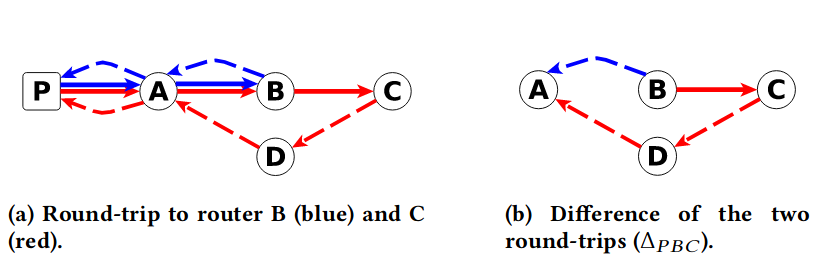
\includegraphics[width=0.7\linewidth]{illustrations/rtt-differ}
	\caption{(a) Le RTT entre la sonde P et les routeurs B et C. (b) La différence entre les  chemins de retour depuis les routeurs B et C vers la sonde P. Source : \cite{DBLP:journals/corr/FontugneAPB16}}
	\label{fig:rtt-differ}
\end{figure}

\paragraph{Le principe de la détection des changements des délais}~

L'évolution du délai d'un lien est déduit de l'évolution de son RTT différentiel. Reprenons d'abord l'équation (\ref{eq:rttdiff}) du RTT différentiel du lien BC :   $\delta_{BC}$ + $\varepsilon_{PBC}$. 
 
La valeur de  $\delta_{BC}$ dépend de l'état des deux routeurs B et C et ne dépend pas de la sonde P. Tandis que la valeur de $\varepsilon_{PBC}$ dépend de la sonde P; la destination des deux chemin de retours.
 
 Supposons qu'on dispose d'un nombre $n$ de sondes Atlas P$_i$, $i$ $\in$ [$1$, $n$], telles que toutes les sondes ont un chemin de retour  $\varepsilon_{P_{i}BC}$ différent depuis B et depuis C.  Les $n$ RTTs différentiels $\Delta_{P{_i}BC}$ du lien $BC$ pour chacune des sondes $P_i$  partagent la même composante $\delta_{BC}$ :
 
 
 \begin{align*}
 \Delta_{P_{1}BC} &= \delta_{BC} + \varepsilon_{P_{1}BC}\\
  \Delta_{P_{2}BC} &= \delta_{BC} + \varepsilon_{P_{2}BC}\\
  .... &   ... \\
   \Delta_{P_{i}BC} &= \delta_{BC} + \varepsilon_{P_{i}BC}\\
      \Delta_{P_{n}BC} &= \delta_{BC} + \varepsilon_{P_{n}BC}\\
 \end{align*}
 
Les valeurs de  $\varepsilon_{P_{i}BC}$ sont  indépendantes. L'indépendance de ces valeurs implique que la distribution $\Delta_{P_{i}BC}$ est estimé  stable au cours du temps si $\delta_{BC}$ est constant. Toutefois, un changement significatif de la valeur de $\delta_{BC}$ influence les valuers des RTTs différentiels, ainsi,  la distribution des RTTs différentiels $\Delta_{P_{i}BC}$ change. D'où l'idée de l'évolution du délai d'un lien est déduit de l'évolution de son RTT différentiel.

%Enfin, les changements des délais sont déduits des changements des RTTs différentiel qu'on peut les quantifier.

La détection des anomalies dans les délais repose sur le théorème  central limite (TCL). Ce théorème  annonce que si on a une suite de variables aléatoires $X_i$ indépendantes ayant la même espérance $\mu$ et la même variance $\sigma^2$, la moyenne de ces variables aléatoires est une variable aléatoire qui suit une loi normale. Ce théorème a été utilisé pour calculer la médiane des RTTs différentiels d'un lien d'une période $d_k$. Les auteurs du travail de référence ont ajusté ce théorème, ils ont utilisé la médiane au lieu de la moyenne. Cet ajustement  a été validé en évaluant les performances de la moyenne ainsi que de la médiane sur des échantillons des RTTs différentiels des liens  dont ils connaissent leur état en matière de délais.

%De manière générale, le théorème central limite explique la distribution des moyennes des échantillons. Ce théorème peut être appliquer aux différents lois. Par exemple la loi normale \footnote{Un exemple illustratif dans \ref{appendix:clt-exemple}.}, binomiale, etc. 



\section{L'étude des délais des liens en pratique : l'évolution du RTT différentiel des liens}

L'évolution des RTTs différentiels est une des applications du principe décrit dans la section  \ref{principe-de-detection}. Pour un lien donné, le suivi s'étale sur plusieurs  périodes. En plus du suivi du RTT différentiel, il y a aussi l'identification d'éventuelles anomalies pour ce lien.


\subsection{Les étapes principales de détection} \label{steps:detection}
Les étapes du processus de détection peuvent être résumées dans les éléments suivants:

\begin{enumerate}[label=(\roman*)]
	
	\item Vérification de la validité de tout traceroute.
	
	\item Calcul des RTTs différentiels de chaque lien identifié dans les traceroutes.

	\item Caractérisation des liens avec le théorème central limite (CLT).
	
	\item  Comparaison de l'état de chaque lien avec sa référence  et l'identification des anomalies.

	\item Mise à jour de la référence du lien.
\end{enumerate}
\subsection{Description des paramètres de l'analyse des délais} \label{par:parametre-de-lanalyse}~

La détection des changements des délais nécessite l'ajustement d'un nombre de paramètres. Ces paramètres ont des valeurs par défaut définies dans le travail de référence. 
%, La valeur de chaque paramètre est relative au  fondement utilisé théorique ou bien empirique, qui a été  justifié par les auteurs du travail de référence.   
Ci-dessous les paramètres à ajuster afin d'obtenir l'évolution des RTTs différentiels d'un lien ainsi que les éventuelles anomalies.  

\begin{description}
	
	\item[traceroutes] : ce sont l'ensemble des résultats de requêtes traceroute. La détection des anomalies est effectuée suivant le nombre de traceroutes analysés et la période précisée. Les  traceroutes sont obtenus en utilisant l'API fournie par RIPE Atlas.
	
	\item[start] : c'est la date de début de l'analyse. Seuls les traceroutes effectués par les sondes Atlas à partir de cette date qui sont analysés.

\item[end]  : c'est la date marquant la fin de l'analyse. Comme le paramètre \textit{start}, c'est la date maximales des  traceroutes effectués par les sondes Atlas à considérer.

\item[timeWindow]:  ce paramètre est exprimé en secondes. Il correspond à la durée des périodes de l'analyse. Ces périodes ont la même durée. Autrement dit, la durée entre   \textit{start} et \textit{end} est divisée sur
 cette même taille: \textit{timeWindow}, c'est qui est illustré dans la Figure  \ref{fig:timing_tex}. Par défaut, \textit{timeWindow} a $ 3600 $ secondes comme valeur.

%illustre le contexte des trois paramètres \textit{start}, \textit{end} et \textit{timeWindow} avec les étapes principales.



\begin{figure}[h]
	\centering
	\captionsetup{justification=centering}
	% Graphic for TeX using PGF
% Title: /home/hayat/RipeAtlasTraceroutesAnalysis/report/illustrations/timing.dia
% Creator: Dia v0.97+git
% CreationDate: Mon Dec  3 23:19:01 2018
% For: hayat
% \usepackage{tikz}
% The following commands are not supported in PSTricks at present
% We define them conditionally, so when they are implemented,
% this pgf file will use them.
\ifx\du\undefined
  \newlength{\du}
\fi
\setlength{\du}{15\unitlength}
\begin{tikzpicture}[even odd rule]
\pgftransformxscale{1.000000}
\pgftransformyscale{-1.000000}
\definecolor{dialinecolor}{rgb}{0.000000, 0.000000, 0.000000}
\pgfsetstrokecolor{dialinecolor}
\pgfsetstrokeopacity{1.000000}
\definecolor{diafillcolor}{rgb}{1.000000, 1.000000, 1.000000}
\pgfsetfillcolor{diafillcolor}
\pgfsetfillopacity{1.000000}
\pgfsetlinewidth{0.100000\du}
\pgfsetdash{}{0pt}
\pgfsetbuttcap
{
\definecolor{diafillcolor}{rgb}{0.000000, 0.000000, 0.000000}
\pgfsetfillcolor{diafillcolor}
\pgfsetfillopacity{1.000000}
% was here!!!
}
\definecolor{dialinecolor}{rgb}{0.000000, 0.000000, 0.000000}
\pgfsetstrokecolor{dialinecolor}
\pgfsetstrokeopacity{1.000000}
\draw (34.600000\du,6.050000\du)--(40.550000\du,6.000000\du);
\pgfsetlinewidth{0.100000\du}
\pgfsetdash{}{0pt}
\pgfsetmiterjoin
\pgfsetbuttcap
\definecolor{dialinecolor}{rgb}{0.000000, 0.000000, 0.000000}
\pgfsetstrokecolor{dialinecolor}
\pgfsetstrokeopacity{1.000000}
\draw (35.097882\du,5.795807\du)--(35.102083\du,6.295790\du);
\pgfsetlinewidth{0.100000\du}
\pgfsetdash{}{0pt}
\pgfsetmiterjoin
\pgfsetbuttcap
\definecolor{dialinecolor}{rgb}{0.000000, 0.000000, 0.000000}
\pgfsetstrokecolor{dialinecolor}
\pgfsetstrokeopacity{1.000000}
\draw (40.052118\du,6.254193\du)--(40.047917\du,5.754210\du);
% setfont left to latex
\definecolor{dialinecolor}{rgb}{0.000000, 0.000000, 0.000000}
\pgfsetstrokecolor{dialinecolor}
\pgfsetstrokeopacity{1.000000}
\definecolor{diafillcolor}{rgb}{0.000000, 0.000000, 0.000000}
\pgfsetfillcolor{diafillcolor}
\pgfsetfillopacity{1.000000}
\node[anchor=base west,inner sep=0pt,outer sep=0pt,color=dialinecolor] at (14.800200\du,8.464650\du){start};
% setfont left to latex
\definecolor{dialinecolor}{rgb}{0.000000, 0.000000, 0.000000}
\pgfsetstrokecolor{dialinecolor}
\pgfsetstrokeopacity{1.000000}
\definecolor{diafillcolor}{rgb}{0.000000, 0.000000, 0.000000}
\pgfsetfillcolor{diafillcolor}
\pgfsetfillopacity{1.000000}
\node[anchor=base west,inner sep=0pt,outer sep=0pt,color=dialinecolor] at (39.375600\du,7.990890\du){end};
% setfont left to latex
\definecolor{dialinecolor}{rgb}{0.000000, 0.000000, 0.000000}
\pgfsetstrokecolor{dialinecolor}
\pgfsetstrokeopacity{1.000000}
\definecolor{diafillcolor}{rgb}{0.000000, 0.000000, 0.000000}
\pgfsetfillcolor{diafillcolor}
\pgfsetfillopacity{1.000000}
\node[anchor=base west,inner sep=0pt,outer sep=0pt,color=dialinecolor] at (24.374800\du,8.977310\du){Périodes de l'analyse};
% setfont left to latex
\definecolor{dialinecolor}{rgb}{0.000000, 0.000000, 0.000000}
\pgfsetstrokecolor{dialinecolor}
\pgfsetstrokeopacity{1.000000}
\definecolor{diafillcolor}{rgb}{0.000000, 0.000000, 0.000000}
\pgfsetfillcolor{diafillcolor}
\pgfsetfillopacity{1.000000}
\node[anchor=base west,inner sep=0pt,outer sep=0pt,color=dialinecolor] at (14.950000\du,7.200000\du){d1};
\pgfsetlinewidth{0.100000\du}
\pgfsetdash{}{0pt}
\pgfsetbuttcap
{
\definecolor{diafillcolor}{rgb}{0.000000, 0.000000, 0.000000}
\pgfsetfillcolor{diafillcolor}
\pgfsetfillopacity{1.000000}
% was here!!!
}
\definecolor{dialinecolor}{rgb}{0.000000, 0.000000, 0.000000}
\pgfsetstrokecolor{dialinecolor}
\pgfsetstrokeopacity{1.000000}
\draw (29.656800\du,6.066270\du)--(35.606800\du,6.016270\du);
\pgfsetlinewidth{0.100000\du}
\pgfsetdash{}{0pt}
\pgfsetmiterjoin
\pgfsetbuttcap
\definecolor{dialinecolor}{rgb}{0.000000, 0.000000, 0.000000}
\pgfsetstrokecolor{dialinecolor}
\pgfsetstrokeopacity{1.000000}
\draw (30.154682\du,5.812077\du)--(30.158883\du,6.312060\du);
\pgfsetlinewidth{0.100000\du}
\pgfsetdash{}{0pt}
\pgfsetmiterjoin
\pgfsetbuttcap
\definecolor{dialinecolor}{rgb}{0.000000, 0.000000, 0.000000}
\pgfsetstrokecolor{dialinecolor}
\pgfsetstrokeopacity{1.000000}
\draw (35.108918\du,6.270463\du)--(35.104717\du,5.770480\du);
\pgfsetlinewidth{0.100000\du}
\pgfsetdash{}{0pt}
\pgfsetbuttcap
{
\definecolor{diafillcolor}{rgb}{0.000000, 0.000000, 0.000000}
\pgfsetfillcolor{diafillcolor}
\pgfsetfillopacity{1.000000}
% was here!!!
}
\definecolor{dialinecolor}{rgb}{0.000000, 0.000000, 0.000000}
\pgfsetstrokecolor{dialinecolor}
\pgfsetstrokeopacity{1.000000}
\draw (24.701800\du,6.106100\du)--(30.651800\du,6.056100\du);
\pgfsetlinewidth{0.100000\du}
\pgfsetdash{}{0pt}
\pgfsetmiterjoin
\pgfsetbuttcap
\definecolor{dialinecolor}{rgb}{0.000000, 0.000000, 0.000000}
\pgfsetstrokecolor{dialinecolor}
\pgfsetstrokeopacity{1.000000}
\draw (25.199682\du,5.851907\du)--(25.203883\du,6.351890\du);
\pgfsetlinewidth{0.100000\du}
\pgfsetdash{}{0pt}
\pgfsetmiterjoin
\pgfsetbuttcap
\definecolor{dialinecolor}{rgb}{0.000000, 0.000000, 0.000000}
\pgfsetstrokecolor{dialinecolor}
\pgfsetstrokeopacity{1.000000}
\draw (30.153918\du,6.310293\du)--(30.149717\du,5.810310\du);
\pgfsetlinewidth{0.100000\du}
\pgfsetdash{}{0pt}
\pgfsetbuttcap
{
\definecolor{diafillcolor}{rgb}{0.000000, 0.000000, 0.000000}
\pgfsetfillcolor{diafillcolor}
\pgfsetfillopacity{1.000000}
% was here!!!
}
\definecolor{dialinecolor}{rgb}{0.000000, 0.000000, 0.000000}
\pgfsetstrokecolor{dialinecolor}
\pgfsetstrokeopacity{1.000000}
\draw (19.796600\du,6.121020\du)--(25.746600\du,6.071020\du);
\pgfsetlinewidth{0.100000\du}
\pgfsetdash{}{0pt}
\pgfsetmiterjoin
\pgfsetbuttcap
\definecolor{dialinecolor}{rgb}{0.000000, 0.000000, 0.000000}
\pgfsetstrokecolor{dialinecolor}
\pgfsetstrokeopacity{1.000000}
\draw (20.294482\du,5.866827\du)--(20.298683\du,6.366810\du);
\pgfsetlinewidth{0.100000\du}
\pgfsetdash{}{0pt}
\pgfsetmiterjoin
\pgfsetbuttcap
\definecolor{dialinecolor}{rgb}{0.000000, 0.000000, 0.000000}
\pgfsetstrokecolor{dialinecolor}
\pgfsetstrokeopacity{1.000000}
\draw (25.248718\du,6.325213\du)--(25.244517\du,5.825230\du);
\pgfsetlinewidth{0.100000\du}
\pgfsetdash{}{0pt}
\pgfsetbuttcap
{
\definecolor{diafillcolor}{rgb}{0.000000, 0.000000, 0.000000}
\pgfsetfillcolor{diafillcolor}
\pgfsetfillopacity{1.000000}
% was here!!!
}
\definecolor{dialinecolor}{rgb}{0.000000, 0.000000, 0.000000}
\pgfsetstrokecolor{dialinecolor}
\pgfsetstrokeopacity{1.000000}
\draw (14.841600\du,6.135940\du)--(20.791600\du,6.085940\du);
\pgfsetlinewidth{0.100000\du}
\pgfsetdash{}{0pt}
\pgfsetmiterjoin
\pgfsetbuttcap
\definecolor{dialinecolor}{rgb}{0.000000, 0.000000, 0.000000}
\pgfsetstrokecolor{dialinecolor}
\pgfsetstrokeopacity{1.000000}
\draw (15.339482\du,5.881747\du)--(15.343683\du,6.381730\du);
\pgfsetlinewidth{0.100000\du}
\pgfsetdash{}{0pt}
\pgfsetmiterjoin
\pgfsetbuttcap
\definecolor{dialinecolor}{rgb}{0.000000, 0.000000, 0.000000}
\pgfsetstrokecolor{dialinecolor}
\pgfsetstrokeopacity{1.000000}
\draw (20.293718\du,6.340133\du)--(20.289517\du,5.840150\du);
% setfont left to latex
\definecolor{dialinecolor}{rgb}{0.000000, 0.000000, 0.000000}
\pgfsetstrokecolor{dialinecolor}
\pgfsetstrokeopacity{1.000000}
\definecolor{diafillcolor}{rgb}{0.000000, 0.000000, 0.000000}
\pgfsetfillcolor{diafillcolor}
\pgfsetfillopacity{1.000000}
\node[anchor=base west,inner sep=0pt,outer sep=0pt,color=dialinecolor] at (19.845000\du,7.235000\du){d2};
% setfont left to latex
\definecolor{dialinecolor}{rgb}{0.000000, 0.000000, 0.000000}
\pgfsetstrokecolor{dialinecolor}
\pgfsetstrokeopacity{1.000000}
\definecolor{diafillcolor}{rgb}{0.000000, 0.000000, 0.000000}
\pgfsetfillcolor{diafillcolor}
\pgfsetfillopacity{1.000000}
\node[anchor=base west,inner sep=0pt,outer sep=0pt,color=dialinecolor] at (24.750000\du,7.300000\du){d3};
% setfont left to latex
\definecolor{dialinecolor}{rgb}{0.000000, 0.000000, 0.000000}
\pgfsetstrokecolor{dialinecolor}
\pgfsetstrokeopacity{1.000000}
\definecolor{diafillcolor}{rgb}{0.000000, 0.000000, 0.000000}
\pgfsetfillcolor{diafillcolor}
\pgfsetfillopacity{1.000000}
\node[anchor=base west,inner sep=0pt,outer sep=0pt,color=dialinecolor] at (29.740000\du,7.175000\du){di};
% setfont left to latex
\definecolor{dialinecolor}{rgb}{0.000000, 0.000000, 0.000000}
\pgfsetstrokecolor{dialinecolor}
\pgfsetstrokeopacity{1.000000}
\definecolor{diafillcolor}{rgb}{0.000000, 0.000000, 0.000000}
\pgfsetfillcolor{diafillcolor}
\pgfsetfillopacity{1.000000}
\node[anchor=base west,inner sep=0pt,outer sep=0pt,color=dialinecolor] at (34.685000\du,7.165000\du){di+1};
\pgfsetlinewidth{0.100000\du}
\pgfsetdash{}{0pt}
\pgfsetbuttcap
\definecolor{dialinecolor}{rgb}{0.000000, 0.000000, 0.000000}
\pgfsetstrokecolor{dialinecolor}
\pgfsetstrokeopacity{1.000000}
\pgfpathmoveto{\pgfpoint{25.180033\du}{4.900033\du}}
\pgfpatharc{315}{226}{3.501250\du and 3.501250\du}
\pgfusepath{stroke}
% setfont left to latex
\definecolor{dialinecolor}{rgb}{0.000000, 0.000000, 0.000000}
\pgfsetstrokecolor{dialinecolor}
\pgfsetstrokeopacity{1.000000}
\definecolor{diafillcolor}{rgb}{0.000000, 0.000000, 0.000000}
\pgfsetfillcolor{diafillcolor}
\pgfsetfillopacity{1.000000}
\node[anchor=base west,inner sep=0pt,outer sep=0pt,color=dialinecolor] at (20.780000\du,3.400000\du){timeWindow};
\pgfsetlinewidth{0.100000\du}
\pgfsetdash{}{0pt}
\pgfsetbuttcap
\definecolor{dialinecolor}{rgb}{0.000000, 0.000000, 0.000000}
\pgfsetstrokecolor{dialinecolor}
\pgfsetstrokeopacity{1.000000}
\pgfpathmoveto{\pgfpoint{29.975033\du}{4.885033\du}}
\pgfpatharc{315}{226}{3.501250\du and 3.501250\du}
\pgfusepath{stroke}
% setfont left to latex
\definecolor{dialinecolor}{rgb}{0.000000, 0.000000, 0.000000}
\pgfsetstrokecolor{dialinecolor}
\pgfsetstrokeopacity{1.000000}
\definecolor{diafillcolor}{rgb}{0.000000, 0.000000, 0.000000}
\pgfsetfillcolor{diafillcolor}
\pgfsetfillopacity{1.000000}
\node[anchor=base west,inner sep=0pt,outer sep=0pt,color=dialinecolor] at (25.675000\du,3.485000\du){timeWindow};
\pgfsetlinewidth{0.100000\du}
\pgfsetdash{}{0pt}
\pgfsetbuttcap
\definecolor{dialinecolor}{rgb}{0.000000, 0.000000, 0.000000}
\pgfsetstrokecolor{dialinecolor}
\pgfsetstrokeopacity{1.000000}
\pgfpathmoveto{\pgfpoint{20.275033\du}{4.785033\du}}
\pgfpatharc{315}{226}{3.501250\du and 3.501250\du}
\pgfusepath{stroke}
% setfont left to latex
\definecolor{dialinecolor}{rgb}{0.000000, 0.000000, 0.000000}
\pgfsetstrokecolor{dialinecolor}
\pgfsetstrokeopacity{1.000000}
\definecolor{diafillcolor}{rgb}{0.000000, 0.000000, 0.000000}
\pgfsetfillcolor{diafillcolor}
\pgfsetfillopacity{1.000000}
\node[anchor=base west,inner sep=0pt,outer sep=0pt,color=dialinecolor] at (16.025000\du,3.435000\du){timeWindow};
\end{tikzpicture}

	\caption{Illustration des périodes de l'analyse entre la date de début et la date de fin}
	\label{fig:timing_tex}
\end{figure}
%\begin{figure}[h]	
%	\centering
%	\resizebox{\textwidth}{!}{
%		% Graphic for TeX using PGF
% Title: /home/bellafkih/Documents/2018-2019/memoire/rapport_memoire/dia/timewindow.dia
% Creator: Dia v0.97.3
% CreationDate: Sun Oct  7 15:34:20 2018
% For: bellafkih
% \usepackage{tikz}
% The following commands are not supported in PSTricks at present
% We define them conditionally, so when they are implemented,
% this pgf file will use them.
\ifx\du\undefined
  \newlength{\du}
\fi
\setlength{\du}{15\unitlength}
\begin{tikzpicture}
\pgftransformxscale{1.000000}
\pgftransformyscale{-1.000000}
\definecolor{dialinecolor}{rgb}{0.000000, 0.000000, 0.000000}
\pgfsetstrokecolor{dialinecolor}
\definecolor{dialinecolor}{rgb}{1.000000, 1.000000, 1.000000}
\pgfsetfillcolor{dialinecolor}
\pgfsetlinewidth{0.200000\du}
\pgfsetdash{}{0pt}
\pgfsetdash{}{0pt}
\pgfsetbuttcap
{
\definecolor{dialinecolor}{rgb}{0.000000, 0.000000, 0.000000}
\pgfsetfillcolor{dialinecolor}
% was here!!!
\pgfsetarrowsend{to}
\definecolor{dialinecolor}{rgb}{0.000000, 0.000000, 0.000000}
\pgfsetstrokecolor{dialinecolor}
\draw (10.000000\du,2.000000\du)--(10.000000\du,26.650000\du);
}
% setfont left to latex
\definecolor{dialinecolor}{rgb}{0.000000, 0.000000, 0.000000}
\pgfsetstrokecolor{dialinecolor}
\node[anchor=west] at (7.650000\du,2.050000\du){start};
% setfont left to latex
\definecolor{dialinecolor}{rgb}{0.000000, 0.000000, 0.000000}
\pgfsetstrokecolor{dialinecolor}
\node[anchor=west] at (7.850000\du,22.100000\du){end};
\pgfsetlinewidth{0.000000\du}
\pgfsetdash{}{0pt}
\pgfsetdash{}{0pt}
\pgfsetbuttcap
{
\definecolor{dialinecolor}{rgb}{0.000000, 0.000000, 0.000000}
\pgfsetfillcolor{dialinecolor}
% was here!!!
\definecolor{dialinecolor}{rgb}{0.000000, 0.000000, 0.000000}
\pgfsetstrokecolor{dialinecolor}
\draw (10.600000\du,2.000000\du)--(9.450000\du,2.000000\du);
}
\pgfsetlinewidth{0.000000\du}
\pgfsetdash{}{0pt}
\pgfsetdash{}{0pt}
\pgfsetbuttcap
{
\definecolor{dialinecolor}{rgb}{0.000000, 0.000000, 0.000000}
\pgfsetfillcolor{dialinecolor}
% was here!!!
\definecolor{dialinecolor}{rgb}{0.000000, 0.000000, 0.000000}
\pgfsetstrokecolor{dialinecolor}
\draw (10.585000\du,5.960000\du)--(9.435000\du,5.960000\du);
}
\pgfsetlinewidth{0.000000\du}
\pgfsetdash{}{0pt}
\pgfsetdash{}{0pt}
\pgfsetbuttcap
{
\definecolor{dialinecolor}{rgb}{0.000000, 0.000000, 0.000000}
\pgfsetfillcolor{dialinecolor}
% was here!!!
\definecolor{dialinecolor}{rgb}{0.000000, 0.000000, 0.000000}
\pgfsetstrokecolor{dialinecolor}
\draw (10.570000\du,10.020000\du)--(9.420000\du,10.020000\du);
}
\pgfsetlinewidth{0.000000\du}
\pgfsetdash{}{0pt}
\pgfsetdash{}{0pt}
\pgfsetbuttcap
{
\definecolor{dialinecolor}{rgb}{0.000000, 0.000000, 0.000000}
\pgfsetfillcolor{dialinecolor}
% was here!!!
\definecolor{dialinecolor}{rgb}{0.000000, 0.000000, 0.000000}
\pgfsetstrokecolor{dialinecolor}
\draw (10.505000\du,13.930000\du)--(9.355000\du,13.930000\du);
}
\pgfsetlinewidth{0.000000\du}
\pgfsetdash{}{0pt}
\pgfsetdash{}{0pt}
\pgfsetbuttcap
{
\definecolor{dialinecolor}{rgb}{0.000000, 0.000000, 0.000000}
\pgfsetfillcolor{dialinecolor}
% was here!!!
\definecolor{dialinecolor}{rgb}{0.000000, 0.000000, 0.000000}
\pgfsetstrokecolor{dialinecolor}
\draw (10.540000\du,17.940000\du)--(9.390000\du,17.940000\du);
}
\pgfsetlinewidth{0.000000\du}
\pgfsetdash{}{0pt}
\pgfsetdash{}{0pt}
\pgfsetbuttcap
{
\definecolor{dialinecolor}{rgb}{0.000000, 0.000000, 0.000000}
\pgfsetfillcolor{dialinecolor}
% was here!!!
\definecolor{dialinecolor}{rgb}{0.000000, 0.000000, 0.000000}
\pgfsetstrokecolor{dialinecolor}
\draw (10.575000\du,22.050000\du)--(9.425000\du,22.050000\du);
}
\pgfsetlinewidth{0.000000\du}
\pgfsetdash{}{0pt}
\pgfsetdash{}{0pt}
\pgfsetbuttcap
{
\definecolor{dialinecolor}{rgb}{0.000000, 0.000000, 0.000000}
\pgfsetfillcolor{dialinecolor}
% was here!!!
\pgfsetarrowsstart{to}
\pgfsetarrowsend{to}
\definecolor{dialinecolor}{rgb}{0.000000, 0.000000, 0.000000}
\pgfsetstrokecolor{dialinecolor}
\pgfpathmoveto{\pgfpoint{6.950071\du}{2.049940\du}}
\pgfpatharc{231}{129}{2.448949\du and 2.448949\du}
\pgfusepath{stroke}
}
% setfont left to latex
\definecolor{dialinecolor}{rgb}{0.000000, 0.000000, 0.000000}
\pgfsetstrokecolor{dialinecolor}
\node[anchor=west] at (2.150000\du,26.900000\du){Temps en secondes (s)};
\pgfsetlinewidth{0.000000\du}
\pgfsetdash{}{0pt}
\pgfsetdash{}{0pt}
\pgfsetbuttcap
{
\definecolor{dialinecolor}{rgb}{0.000000, 0.000000, 0.000000}
\pgfsetfillcolor{dialinecolor}
% was here!!!
\pgfsetarrowsstart{to}
\pgfsetarrowsend{to}
\definecolor{dialinecolor}{rgb}{0.000000, 0.000000, 0.000000}
\pgfsetstrokecolor{dialinecolor}
\pgfpathmoveto{\pgfpoint{7.049251\du}{6.119940\du}}
\pgfpatharc{231}{129}{2.448949\du and 2.448949\du}
\pgfusepath{stroke}
}
\pgfsetlinewidth{0.000000\du}
\pgfsetdash{}{0pt}
\pgfsetdash{}{0pt}
\pgfsetbuttcap
{
\definecolor{dialinecolor}{rgb}{0.000000, 0.000000, 0.000000}
\pgfsetfillcolor{dialinecolor}
% was here!!!
\pgfsetarrowsstart{to}
\pgfsetarrowsend{to}
\definecolor{dialinecolor}{rgb}{0.000000, 0.000000, 0.000000}
\pgfsetstrokecolor{dialinecolor}
\pgfpathmoveto{\pgfpoint{6.984251\du}{10.079940\du}}
\pgfpatharc{231}{129}{2.448949\du and 2.448949\du}
\pgfusepath{stroke}
}
\pgfsetlinewidth{0.000000\du}
\pgfsetdash{}{0pt}
\pgfsetdash{}{0pt}
\pgfsetbuttcap
{
\definecolor{dialinecolor}{rgb}{0.000000, 0.000000, 0.000000}
\pgfsetfillcolor{dialinecolor}
% was here!!!
\pgfsetarrowsstart{to}
\pgfsetarrowsend{to}
\definecolor{dialinecolor}{rgb}{0.000000, 0.000000, 0.000000}
\pgfsetstrokecolor{dialinecolor}
\pgfpathmoveto{\pgfpoint{6.869251\du}{14.089940\du}}
\pgfpatharc{231}{129}{2.448949\du and 2.448949\du}
\pgfusepath{stroke}
}
\pgfsetlinewidth{0.000000\du}
\pgfsetdash{}{0pt}
\pgfsetdash{}{0pt}
\pgfsetbuttcap
{
\definecolor{dialinecolor}{rgb}{0.000000, 0.000000, 0.000000}
\pgfsetfillcolor{dialinecolor}
% was here!!!
\pgfsetarrowsstart{to}
\pgfsetarrowsend{to}
\definecolor{dialinecolor}{rgb}{0.000000, 0.000000, 0.000000}
\pgfsetstrokecolor{dialinecolor}
\pgfpathmoveto{\pgfpoint{6.954251\du}{18.099940\du}}
\pgfpatharc{231}{129}{2.448949\du and 2.448949\du}
\pgfusepath{stroke}
}
% setfont left to latex
\definecolor{dialinecolor}{rgb}{0.000000, 0.000000, 0.000000}
\pgfsetstrokecolor{dialinecolor}
\node[anchor=west] at (0.650000\du,4.050000\du){timeWindow s};
% setfont left to latex
\definecolor{dialinecolor}{rgb}{0.000000, 0.000000, 0.000000}
\pgfsetstrokecolor{dialinecolor}
\node[anchor=west] at (0.685100\du,8.005000\du){timeWindow s};
% setfont left to latex
\definecolor{dialinecolor}{rgb}{0.000000, 0.000000, 0.000000}
\pgfsetstrokecolor{dialinecolor}
\node[anchor=west] at (0.870100\du,12.015000\du){timeWindow s};
% setfont left to latex
\definecolor{dialinecolor}{rgb}{0.000000, 0.000000, 0.000000}
\pgfsetstrokecolor{dialinecolor}
\node[anchor=west] at (0.905100\du,16.025000\du){timeWindow s};
% setfont left to latex
\definecolor{dialinecolor}{rgb}{0.000000, 0.000000, 0.000000}
\pgfsetstrokecolor{dialinecolor}
\node[anchor=west] at (1.040100\du,19.935000\du){timeWindow s};
% setfont left to latex
\definecolor{dialinecolor}{rgb}{0.000000, 0.000000, 0.000000}
\pgfsetstrokecolor{dialinecolor}
\node[anchor=west] at (11.200100\du,3.850000\du){appliquer : computeRtt(), mergeRttResults(), outlierDetection()};
% setfont left to latex
\definecolor{dialinecolor}{rgb}{0.000000, 0.000000, 0.000000}
\pgfsetstrokecolor{dialinecolor}
\node[anchor=west] at (11.035100\du,7.905000\du){appliquer : computeRtt(), mergeRttResults(), outlierDetection()};
% setfont left to latex
\definecolor{dialinecolor}{rgb}{0.000000, 0.000000, 0.000000}
\pgfsetstrokecolor{dialinecolor}
\node[anchor=west] at (11.120100\du,12.015000\du){appliquer : computeRtt(), mergeRttResults(), outlierDetection()};
% setfont left to latex
\definecolor{dialinecolor}{rgb}{0.000000, 0.000000, 0.000000}
\pgfsetstrokecolor{dialinecolor}
\node[anchor=west] at (11.105100\du,15.875000\du){appliquer : computeRtt(), mergeRttResults(), outlierDetection()};
% setfont left to latex
\definecolor{dialinecolor}{rgb}{0.000000, 0.000000, 0.000000}
\pgfsetstrokecolor{dialinecolor}
\node[anchor=west] at (11.040100\du,19.885000\du){appliquer : computeRtt(), mergeRttResults(), outlierDetection()};
% setfont left to latex
\definecolor{dialinecolor}{rgb}{0.000000, 0.000000, 0.000000}
\pgfsetstrokecolor{dialinecolor}
\node[anchor=west] at (11.950100\du,2.000000\du){inputs : paramère de l'expérience};
% setfont left to latex
\definecolor{dialinecolor}{rgb}{0.000000, 0.000000, 0.000000}
\pgfsetstrokecolor{dialinecolor}
\node[anchor=west] at (12.050100\du,22.000000\du){output : les changements détéctés et ses caractériqtiques};
\end{tikzpicture}
 
%	}
%	\caption{Illustration du paramètre timeWindow}
%	\label{fig:timewindow}
%\end{figure}

\item[minSeen] : 
%comme l'analyse des liens est réalisée sur plusieurs périodes de durée \textit{timeWindow}, 
ce paramètre est un entier, il indique le déclenchement de la comparaison du RTT différentiel de référence d'un lien avec sa valeur courante.  Par exemple, si $ minSeen = 24 $ et $timeWindow = 3600$ (1 heure), cela implique que la référence de tout lien est construite des valeurs obtenues tout au long la durée $24 * timeWindow$, donc après avoir analysé les traceroutes d'une journée. A la 25\up{ème} \textit{timeWindow}, la détection des anomalies s'effectue.
% nombre de fois à partir desquelles on peut  vérifier son RTT différentiel; s'il indique une anomalie ou non. 
%Par exemple, un lien peut être identifié dans $3$ $d_i$, ou bien être identifié  une seule fois durant toute la période de l'analyse.

\item[alpha ]: noté $\alpha$,  $\alpha \in [0, 1]$, c'est le paramètre de la  moyenne mobile exponentielle calculée.
\guillemotleft \textit{ Les méthodes de lissage exponentiel  sont un ensemble de techniques empiriques de prévision qui accordent plus ou moins d'importance aux valeurs du passé d'une série temporelle\footnote{Source : \url{https://perso.math.univ-toulouse.fr/lagnoux/files/2013/12/Chap6.pdf}, consultée le $30/09/2018.$}}. \guillemotright

 La  moyenne mobile exponentielle est utilisée pour calculer la médiane des RTTs différentiels de référence durant une période $d_k$.
 % Cette médiane constitue une référence  sur laquelle se base la détection des anomalies.
Pour calculer la  valeur de la médiane des RTTs différentiels de référence $ \overline{m}_{t}$   courant la période $ t $ et pour le lien $l$, soit:

\begin{center}
	$ \overline{m}_{t}$ =  $\alpha$ ${m}_{t}$ + (1-  $\alpha$) $ \overline{m}_{t-1}$
\end{center} 

$m_t$ la médiane des RTTs différentiels observée pour $l$ durant le \textit{timeWindow} $t$. 

$ \overline{m}_{t-1}$  la médiane des  RTTs différentiels  de référence durant le \textit{timeWindow} $ t-1 $.  



Pour précision, \{$m_t$\} et \{$ \overline{m}_{t}$\} désignent deux ensembles différents. La taille de chacune de ces deux ensembles est la taille des périodes $d_k$.  Le premier est l'ensemble des médianes des RTTs différentiels de chaque période $d_k$. Or, le deuxième est l'ensemble des médianes des RTTs différentiels construite en utilisant la méthode de la moyenne mobile exponentielle. Le calcul de cette dernière prend en compte les médianes des RTTs différentiels précédentes ainsi que la médiane des RTTs différentiels courante. La participation de ces dernières dans le calcul de la référence est dirigé par le paramètre $\alpha$. 
%La  valeur de la médiane de référence  $ \overline{m}_{t}$ de la période $t$ est obtenue par: 



Le paramètre $\alpha$  contrôle l'importance  des mesures précédentes par rapport aux mesures récentes. De ce fait, \guillemotleft \textit{plus $\alpha$ est proche de $ 1 $ plus les observations récentes influent sur la prévision, à l'inverse un $\alpha$ proche de $0$ conduit à une prévision très stable prenant en compte un passé lointain}.\guillemotright\cite{Lissages-Exponentiels}.  Dans le travail de référence, le paramètre $\alpha$  prend par défaut $0.01$ comme valeur.


\item[confInterval] : l'intervalle de confiance  est défini comme représentant les valeurs probables que peut prendre une moyenne, si l'on accepte une marge d'erreur définie à l'avance à travers la valeur de la marge d'erreur. Il existe plusieurs méthodes pour calculer l'intervalle de confiance d'une proportion. Parmi les critères impliqués sur le choix de la méthode de calcul, on note le nombre total d'expériences.

le RTT différentiel courant et  celui de référence d'un lien donné sont représentés, en pratique, par des intervalles de confiance.  le calcul des intervalles de confiance  est approché par le score de Wilson. Le score de wilson a été adopté car il donne des résultats même si la distribution pour laquelle l'intervalle de confiance est calculé est petite. Pour chaque lien et pour chaque période $d_k$,  deux intervalles de confiances sont calculés, pour ensuite évaluer le chevauchement entre ces deux intervalles. L'outil de détection utilise une marge d'erreur égale à  $ 0.05 $.

%Pour ensu On compare le chevauchement entre l'intervalle de confiance de la médiane de référence avec l'intervalle de confiance de la valeur de médiane calculée en cours, d'un lien donné. Afin d'évaluer si la différence entre ces deux intervalles est significative statistiquement. En particulier une différence de $1$ $ms$ est non significative. On distingue trois cas comme illustré par la figure \ref{fig:illustration-cas-intervalles-deconfiance} et la formule \ref{equ:confidenceIntervalle}. 


%\begin{figure}[H]
%	\centering
%	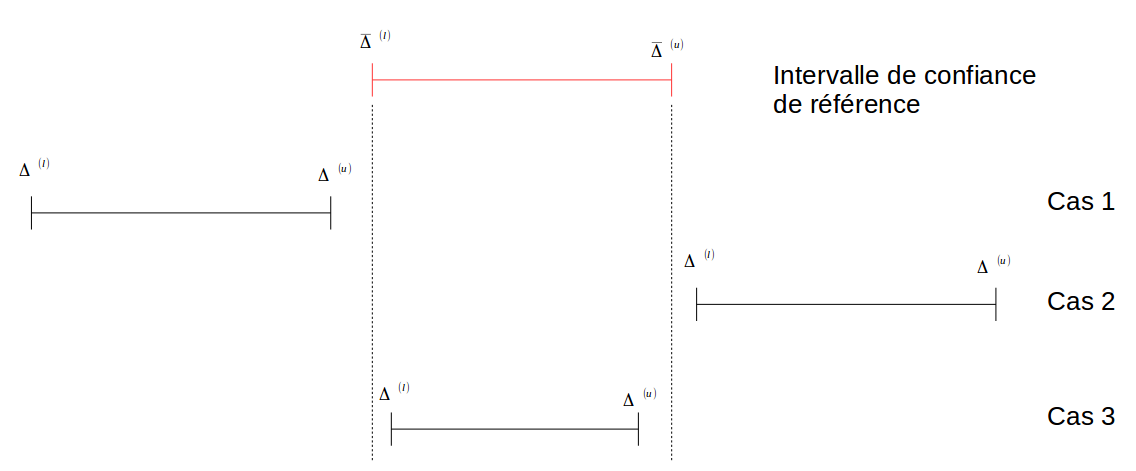
\includegraphics[width=1\linewidth]{illustrations/illustration-cas-intervalles-deconfiance}
%	\caption{La comparaison entre les intervalles de confiance de la médiane de référence et de la médiane calculée.}
%	\label{fig:illustration-cas-intervalles-deconfiance}
%\end{figure}

%Le cas $ 1 $ et $ 2 $ dans la figure 	\ref{fig:illustration-cas-intervalles-deconfiance} illustrent un changement anormal dans le délai du lien en question. Toutefois, le cas $ 3 $ où l'intervalle de confiance courant est inclus dans l'intervalle de référence, est le cas normal, autrement dit,  le délai de ce lien est normal. La différence entre les deux intervalles intervalles de confiance est quantifiée par la déviation $d$ définie par la formule \ref{equ:confidenceIntervalle}.
%
%\begin{equation} \label{equ:confidenceIntervalle}
%d=\begin{cases}
%\frac{\Delta^{(l)} - \overline{\Delta}^{(u)}}{\overline{\Delta}^{(u)} - \overline{\Delta}^{(m)}}    , & \text{if $\overline{\Delta}^{(u)}<\Delta^{(l)}$}.\\
%
%\frac{\overline{\Delta}^{(l)} - \Delta^{(u)}}{\overline{\Delta}^{(u)} - \overline{\Delta}^{(m)}}, & \text{if $\overline{\Delta}^{(m)}<\Delta^{(l)}$}.\\
%0, & \text{otherwise}.
%\end{cases}
%\end{equation}
%
%L'intervalle de confiance est calculé, dans la présente implémentation, avec la fonction  \textit{sm.stats.proportion\_confint}\footnote{Source : \url{https://www.statsmodels.org/dev/generated/statsmodels.stats.proportion.proportion_confint.html}, consultée le $ 07/10/2018 $.}.
%
%\begin{lstlisting}[basicstyle=\tiny]
%statsmodels.stats.proportion.proportion_confint(count, nobs, alpha=0.05, method='normal')
%\end{lstlisting} 
%
%\textit{proportion\_confint} est une implémentation, en python, pour le calcul du score de Wilson. Elle prend les paramètres suivants : 
%\begin{itemize}
%	\item count  : c'est le nombre de fois où une expérience  réussit.
%	\item nobs : c'est le nombre total d'expériences.
%	\item alpha : c'est le paramètre de risque. Généralement il prend les valeurs suivantes $ 5\% $, $ 1\% $ ou $ 0,1\% $. C'est un des paramètres de l'expérience.
%	\item method: on distingue plusieurs méthodes, celle utilisée est \textit{wilson}.
%\end{itemize}
%
%
%En retour, la fonction \textit{proportion\_confint}  fournie \textit{ci\_low} et \textit{ci\_upp}. Ces deux grandeurs sont utilisés pour construire l'intervalle de confiance.
%%, respectivement, ce sont les deux bord de l'intervalle de confiance  avec une probabilité  approximativement de  1-alpha.
%
\end{description}
\subsection{L'évolution du RTT différentiel d'un lien et  la détection des anomalies} \label{rttevolution}

Nous avons décrit les étapes principales de détection dans la section \ref{steps:detection}. Nous  présentons dans ce qui suit  l'algorithme de détection en détail. Les paramètres d'entrée  de cet algorithme sont détaillés dans la section \ref{par:parametre-de-lanalyse}. L'algorithme fournit en résultat l'évolution du RTT différentiel de chaque lien, tout au long de la période de l'analyse, ainsi que son RTT différentiel de référence. Dans le cas d'anomalies détectées, celles-ci sont identifiées tout en précisant la date pendant laquelle l'anomalie a été détectée ainsi que la valeur du RTT différentiel ayant engendré cette anomalie. 

Un traceroute  est un ensemble de sauts $h_i$ dans l'ensemble  $H$ auxquels sont joints l'identifiant de la sonde ayant effectué la requête traceroute et la destination de la requête. Chaque saut est décrit par un ensemble de signaux dans  $S$.  Chaque signal décrit le routeur ayant émis une réponse à la sonde parmi les routeurs traversés avant d'atteindre la destination finale.  Pour le saut $h_i$, on note trois\footnote{Le nombre trois peut varier dans certains cas. L'outil de détection conçu est adapté à tout nombre de signaux.} signaux $s_{i, j},  j\in [1,3]$ dont le routeur émettant le signal est $from_{i,j}$ et son RTT est égal à $rtt_{i,j}$. C'est ce qu'illustre  la Figure \ref{fig:traceroute}.

\begin{figure}[H]
	\centering
	\captionsetup{justification=centering}
	\resizebox{\textwidth}{!}{
	% Graphic for TeX using PGF
% Title: /home/hayat/RipeAtlasTraceroutesAnalysis/report/illustrations/dia/traceroute_.dia
% Creator: Dia v0.97+git
% CreationDate: Fri Dec 28 18:14:49 2018
% For: hayat
% \usepackage{tikz}
% The following commands are not supported in PSTricks at present
% We define them conditionally, so when they are implemented,
% this pgf file will use them.
\ifx\du\undefined
  \newlength{\du}
\fi
\setlength{\du}{15\unitlength}
\begin{tikzpicture}[even odd rule]
\pgftransformxscale{1.000000}
\pgftransformyscale{-1.000000}
\definecolor{dialinecolor}{rgb}{0.000000, 0.000000, 0.000000}
\pgfsetstrokecolor{dialinecolor}
\pgfsetstrokeopacity{1.000000}
\definecolor{diafillcolor}{rgb}{1.000000, 1.000000, 1.000000}
\pgfsetfillcolor{diafillcolor}
\pgfsetfillopacity{1.000000}
\pgfsetlinewidth{0.100000\du}
\pgfsetdash{}{0pt}
\pgfsetmiterjoin
{\pgfsetcornersarced{\pgfpoint{0.000000\du}{0.000000\du}}\definecolor{diafillcolor}{rgb}{1.000000, 1.000000, 1.000000}
\pgfsetfillcolor{diafillcolor}
\pgfsetfillopacity{1.000000}
\fill (2.487500\du,12.100000\du)--(2.487500\du,14.000000\du)--(5.712500\du,14.000000\du)--(5.712500\du,12.100000\du)--cycle;
}{\pgfsetcornersarced{\pgfpoint{0.000000\du}{0.000000\du}}\definecolor{dialinecolor}{rgb}{0.000000, 0.000000, 0.000000}
\pgfsetstrokecolor{dialinecolor}
\pgfsetstrokeopacity{1.000000}
\draw (2.487500\du,12.100000\du)--(2.487500\du,14.000000\du)--(5.712500\du,14.000000\du)--(5.712500\du,12.100000\du)--cycle;
}% setfont left to latex
\definecolor{dialinecolor}{rgb}{0.000000, 0.000000, 0.000000}
\pgfsetstrokecolor{dialinecolor}
\pgfsetstrokeopacity{1.000000}
\definecolor{diafillcolor}{rgb}{0.000000, 0.000000, 0.000000}
\pgfsetfillcolor{diafillcolor}
\pgfsetfillopacity{1.000000}
\node[anchor=base,inner sep=0pt, outer sep=0pt,color=dialinecolor] at (4.100000\du,13.245000\du){source};
\pgfsetlinewidth{0.100000\du}
\pgfsetdash{}{0pt}
\pgfsetmiterjoin
{\pgfsetcornersarced{\pgfpoint{0.000000\du}{0.000000\du}}\definecolor{diafillcolor}{rgb}{1.000000, 1.000000, 1.000000}
\pgfsetfillcolor{diafillcolor}
\pgfsetfillopacity{1.000000}
\fill (46.257500\du,11.850000\du)--(46.257500\du,13.750000\du)--(50.942500\du,13.750000\du)--(50.942500\du,11.850000\du)--cycle;
}{\pgfsetcornersarced{\pgfpoint{0.000000\du}{0.000000\du}}\definecolor{dialinecolor}{rgb}{0.000000, 0.000000, 0.000000}
\pgfsetstrokecolor{dialinecolor}
\pgfsetstrokeopacity{1.000000}
\draw (46.257500\du,11.850000\du)--(46.257500\du,13.750000\du)--(50.942500\du,13.750000\du)--(50.942500\du,11.850000\du)--cycle;
}% setfont left to latex
\definecolor{dialinecolor}{rgb}{0.000000, 0.000000, 0.000000}
\pgfsetstrokecolor{dialinecolor}
\pgfsetstrokeopacity{1.000000}
\definecolor{diafillcolor}{rgb}{0.000000, 0.000000, 0.000000}
\pgfsetfillcolor{diafillcolor}
\pgfsetfillopacity{1.000000}
\node[anchor=base,inner sep=0pt, outer sep=0pt,color=dialinecolor] at (48.600000\du,12.995000\du){destination};
\pgfsetlinewidth{0.100000\du}
\pgfsetdash{}{0pt}
\pgfsetmiterjoin
\definecolor{diafillcolor}{rgb}{1.000000, 1.000000, 1.000000}
\pgfsetfillcolor{diafillcolor}
\pgfsetfillopacity{1.000000}
\pgfpathellipse{\pgfpoint{11.648369\du}{12.925048\du}}{\pgfpoint{1.195569\du}{0\du}}{\pgfpoint{0\du}{1.078448\du}}
\pgfusepath{fill}
\definecolor{dialinecolor}{rgb}{0.000000, 0.000000, 0.000000}
\pgfsetstrokecolor{dialinecolor}
\pgfsetstrokeopacity{1.000000}
\pgfpathellipse{\pgfpoint{11.648369\du}{12.925048\du}}{\pgfpoint{1.195569\du}{0\du}}{\pgfpoint{0\du}{1.078448\du}}
\pgfusepath{stroke}
% setfont left to latex
\definecolor{dialinecolor}{rgb}{0.000000, 0.000000, 0.000000}
\pgfsetstrokecolor{dialinecolor}
\pgfsetstrokeopacity{1.000000}
\definecolor{diafillcolor}{rgb}{0.000000, 0.000000, 0.000000}
\pgfsetfillcolor{diafillcolor}
\pgfsetfillopacity{1.000000}
\node[anchor=base,inner sep=0pt, outer sep=0pt,color=dialinecolor] at (11.648369\du,13.120048\du){R1};
\pgfsetlinewidth{0.100000\du}
\pgfsetdash{}{0pt}
\pgfsetmiterjoin
\definecolor{diafillcolor}{rgb}{1.000000, 1.000000, 1.000000}
\pgfsetfillcolor{diafillcolor}
\pgfsetfillopacity{1.000000}
\pgfpathellipse{\pgfpoint{26.640569\du}{13.018448\du}}{\pgfpoint{1.195569\du}{0\du}}{\pgfpoint{0\du}{1.078448\du}}
\pgfusepath{fill}
\definecolor{dialinecolor}{rgb}{0.000000, 0.000000, 0.000000}
\pgfsetstrokecolor{dialinecolor}
\pgfsetstrokeopacity{1.000000}
\pgfpathellipse{\pgfpoint{26.640569\du}{13.018448\du}}{\pgfpoint{1.195569\du}{0\du}}{\pgfpoint{0\du}{1.078448\du}}
\pgfusepath{stroke}
% setfont left to latex
\definecolor{dialinecolor}{rgb}{0.000000, 0.000000, 0.000000}
\pgfsetstrokecolor{dialinecolor}
\pgfsetstrokeopacity{1.000000}
\definecolor{diafillcolor}{rgb}{0.000000, 0.000000, 0.000000}
\pgfsetfillcolor{diafillcolor}
\pgfsetfillopacity{1.000000}
\node[anchor=base,inner sep=0pt, outer sep=0pt,color=dialinecolor] at (26.640569\du,13.213448\du){R2};
\pgfsetlinewidth{0.100000\du}
\pgfsetdash{}{0pt}
\pgfsetbuttcap
{
\definecolor{diafillcolor}{rgb}{0.000000, 0.000000, 0.000000}
\pgfsetfillcolor{diafillcolor}
\pgfsetfillopacity{1.000000}
% was here!!!
\definecolor{dialinecolor}{rgb}{0.000000, 0.000000, 0.000000}
\pgfsetstrokecolor{dialinecolor}
\pgfsetstrokeopacity{1.000000}
\draw (5.750239\du,13.017555\du)--(10.452800\du,12.925100\du);
}
\pgfsetlinewidth{0.100000\du}
\pgfsetdash{}{0pt}
\pgfsetbuttcap
{
\definecolor{diafillcolor}{rgb}{0.000000, 0.000000, 0.000000}
\pgfsetfillcolor{diafillcolor}
\pgfsetfillopacity{1.000000}
% was here!!!
\definecolor{dialinecolor}{rgb}{0.000000, 0.000000, 0.000000}
\pgfsetstrokecolor{dialinecolor}
\pgfsetstrokeopacity{1.000000}
\draw (12.844000\du,12.925100\du)--(25.445000\du,13.018448\du);
}
\pgfsetlinewidth{0.100000\du}
\pgfsetdash{}{0pt}
\pgfsetbuttcap
{
\definecolor{diafillcolor}{rgb}{0.000000, 0.000000, 0.000000}
\pgfsetfillcolor{diafillcolor}
\pgfsetfillopacity{1.000000}
% was here!!!
\definecolor{dialinecolor}{rgb}{0.000000, 0.000000, 0.000000}
\pgfsetstrokecolor{dialinecolor}
\pgfsetstrokeopacity{1.000000}
\draw (39.886138\du,12.818448\du)--(46.257500\du,12.800000\du);
}
% setfont left to latex
\definecolor{dialinecolor}{rgb}{0.000000, 0.000000, 0.000000}
\pgfsetstrokecolor{dialinecolor}
\pgfsetstrokeopacity{1.000000}
\definecolor{diafillcolor}{rgb}{0.000000, 0.000000, 0.000000}
\pgfsetfillcolor{diafillcolor}
\pgfsetfillopacity{1.000000}
\node[anchor=base west,inner sep=0pt,outer sep=0pt,color=dialinecolor] at (9.050000\du,11.000000\du){$ rtt_{1,1} $, $ rtt_{1,2} $, $ rtt_{1,3} $};
% setfont left to latex
\definecolor{dialinecolor}{rgb}{0.000000, 0.000000, 0.000000}
\pgfsetstrokecolor{dialinecolor}
\pgfsetstrokeopacity{1.000000}
\definecolor{diafillcolor}{rgb}{0.000000, 0.000000, 0.000000}
\pgfsetfillcolor{diafillcolor}
\pgfsetfillopacity{1.000000}
\node[anchor=base west,inner sep=0pt,outer sep=0pt,color=dialinecolor] at (23.395000\du,11.035000\du){$ rtt_{2,1} $, $ rtt_{2,2} $, $ rtt_{2,3} $};
\pgfsetlinewidth{0.100000\du}
\pgfsetdash{}{0pt}
\pgfsetmiterjoin
\definecolor{diafillcolor}{rgb}{1.000000, 1.000000, 1.000000}
\pgfsetfillcolor{diafillcolor}
\pgfsetfillopacity{1.000000}
\pgfpathellipse{\pgfpoint{38.690569\du}{12.818448\du}}{\pgfpoint{1.195569\du}{0\du}}{\pgfpoint{0\du}{1.078448\du}}
\pgfusepath{fill}
\definecolor{dialinecolor}{rgb}{0.000000, 0.000000, 0.000000}
\pgfsetstrokecolor{dialinecolor}
\pgfsetstrokeopacity{1.000000}
\pgfpathellipse{\pgfpoint{38.690569\du}{12.818448\du}}{\pgfpoint{1.195569\du}{0\du}}{\pgfpoint{0\du}{1.078448\du}}
\pgfusepath{stroke}
% setfont left to latex
\definecolor{dialinecolor}{rgb}{0.000000, 0.000000, 0.000000}
\pgfsetstrokecolor{dialinecolor}
\pgfsetstrokeopacity{1.000000}
\definecolor{diafillcolor}{rgb}{0.000000, 0.000000, 0.000000}
\pgfsetfillcolor{diafillcolor}
\pgfsetfillopacity{1.000000}
\node[anchor=base,inner sep=0pt, outer sep=0pt,color=dialinecolor] at (38.690569\du,13.013448\du){Ri};
\pgfsetlinewidth{0.100000\du}
\pgfsetdash{{\pgflinewidth}{0.220000\du}}{0cm}
\pgfsetbuttcap
{
\definecolor{diafillcolor}{rgb}{0.000000, 0.000000, 0.000000}
\pgfsetfillcolor{diafillcolor}
\pgfsetfillopacity{1.000000}
% was here!!!
\definecolor{dialinecolor}{rgb}{0.000000, 0.000000, 0.000000}
\pgfsetstrokecolor{dialinecolor}
\pgfsetstrokeopacity{1.000000}
\draw (28.000000\du,13.000000\du)--(37.000000\du,12.950000\du);
}
% setfont left to latex
\definecolor{dialinecolor}{rgb}{0.000000, 0.000000, 0.000000}
\pgfsetstrokecolor{dialinecolor}
\pgfsetstrokeopacity{1.000000}
\definecolor{diafillcolor}{rgb}{0.000000, 0.000000, 0.000000}
\pgfsetfillcolor{diafillcolor}
\pgfsetfillopacity{1.000000}
\node[anchor=base west,inner sep=0pt,outer sep=0pt,color=dialinecolor] at (36.645000\du,10.985000\du){$ rtt_{i,1} $, $ rtt_{i,2} $, $ rtt_{i,3} $};
% setfont left to latex
\definecolor{dialinecolor}{rgb}{0.000000, 0.000000, 0.000000}
\pgfsetstrokecolor{dialinecolor}
\pgfsetstrokeopacity{1.000000}
\definecolor{diafillcolor}{rgb}{0.000000, 0.000000, 0.000000}
\pgfsetfillcolor{diafillcolor}
\pgfsetfillopacity{1.000000}
\node[anchor=base west,inner sep=0pt,outer sep=0pt,color=dialinecolor] at (8.245000\du,10.035000\du){$from_{1,1}$, $from_{1,2}$, $from_{1,3}$};
% setfont left to latex
\definecolor{dialinecolor}{rgb}{0.000000, 0.000000, 0.000000}
\pgfsetstrokecolor{dialinecolor}
\pgfsetstrokeopacity{1.000000}
\definecolor{diafillcolor}{rgb}{0.000000, 0.000000, 0.000000}
\pgfsetfillcolor{diafillcolor}
\pgfsetfillopacity{1.000000}
\node[anchor=base west,inner sep=0pt,outer sep=0pt,color=dialinecolor] at (22.345000\du,9.985000\du){$ from_{2,1} $, $ from_{2,2} $, $ from_{2,3} $};
% setfont left to latex
\definecolor{dialinecolor}{rgb}{0.000000, 0.000000, 0.000000}
\pgfsetstrokecolor{dialinecolor}
\pgfsetstrokeopacity{1.000000}
\definecolor{diafillcolor}{rgb}{0.000000, 0.000000, 0.000000}
\pgfsetfillcolor{diafillcolor}
\pgfsetfillopacity{1.000000}
\node[anchor=base west,inner sep=0pt,outer sep=0pt,color=dialinecolor] at (35.390000\du,9.975000\du){$ from_{i,1} $, $ from_{i,2} $, $ from_{i,3} $};
% setfont left to latex
\definecolor{dialinecolor}{rgb}{0.000000, 0.000000, 0.000000}
\pgfsetstrokecolor{dialinecolor}
\pgfsetstrokeopacity{1.000000}
\definecolor{diafillcolor}{rgb}{0.000000, 0.000000, 0.000000}
\pgfsetfillcolor{diafillcolor}
\pgfsetfillopacity{1.000000}
\node[anchor=base west,inner sep=0pt,outer sep=0pt,color=dialinecolor] at (10.900000\du,9.000000\du){saut $h_1$};
% setfont left to latex
\definecolor{dialinecolor}{rgb}{0.000000, 0.000000, 0.000000}
\pgfsetstrokecolor{dialinecolor}
\pgfsetstrokeopacity{1.000000}
\definecolor{diafillcolor}{rgb}{0.000000, 0.000000, 0.000000}
\pgfsetfillcolor{diafillcolor}
\pgfsetfillopacity{1.000000}
\node[anchor=base west,inner sep=0pt,outer sep=0pt,color=dialinecolor] at (25.195000\du,8.935000\du){saut $h_2$};
% setfont left to latex
\definecolor{dialinecolor}{rgb}{0.000000, 0.000000, 0.000000}
\pgfsetstrokecolor{dialinecolor}
\pgfsetstrokeopacity{1.000000}
\definecolor{diafillcolor}{rgb}{0.000000, 0.000000, 0.000000}
\pgfsetfillcolor{diafillcolor}
\pgfsetfillopacity{1.000000}
\node[anchor=base west,inner sep=0pt,outer sep=0pt,color=dialinecolor] at (37.785000\du,9.015000\du){saut $h_i$};
\end{tikzpicture}

}
	\caption{Illustration des sauts d'un traceroute avec leurs informations}
	\label{fig:traceroute}
\end{figure}

% Sorties : les dates $d_i$ pendant lesquelles des anomalies ont été détectées.
%\begin{center}
%	 $  d_{i+1} $ - $  d_{i} $ = $  d_{j+1} $ - $  d_{j} $ = \textit{step} 
%	 
%	 \textit{step} est la durée d'une période en secondes, $3600$ pour fenêtre d'une heure.
%\end{center}
% pour tout $ i $ et $ j $ dans$  [1,N] $
\subsection{Processus de  détection des anomalies }\label{steps-rtt-analysis}

 Soient $ d_1 $,$  d_2 $, $d_k$, ... $ d_N $ les $N$ périodes entre \textit{start} et \textit{end} avec $k \in [1,N]$. La différence entre le début de la période $ d_{k+1} $ et le début de la période $ d_k $ est égale à $timeWindow$ pour tout $k+1 \leq N $.  

  Le processus de la détection des anomalies passe par plusieurs étapes. D'abord on  regroupe les traceroutes à analyser par période $d_k$ (étape $ 1 $). Ensuite, on prépare les traceroutes de toute  période $d_k$ en y appliquant un nombre d'opérations (étapes  $ 2 $ à $ 6 $). A la fin de la préparation des traceroutes de toutes les périodes, on ne considère que les données qui concernent le lien à suivre. Ce sont les données qui servent à la comparaison  des  délais d'un lien avec les valeurs de référence (étapes $ 7 $ à $9$). Les étapes de détection sont les suivantes:

\paragraph{1. Regroupement des traceroutes } par période $d_k$. En effet, chaque période $d_k$ est associée à un ensemble de traceroutes ayant été effectués entre $d_k$ et $d_{k+1} - 1 $, avec $k \in [1,N]$, $k+1$ $\leq$ $N $ et  $d_k$ est exprimé en secondes (Unix Timestamp). Les étapes  ($ 2 $ à $ 6 $) concernent  les traceroutes de chaque $d_k$.  

\paragraph{2. Vérification de la validité de chaque traceroute.} 
Les traceroutes sont filtrés en prenant en considération  les points suivants:
\begin{itemize}
	\item élimination des traceroutes échoués complètement;
	\item élimination des signaux contenant une adresse IP privée;
	\item élimination des signaux qui ne contiennent pas un RTT ou  qui contiennent un RTT négatif;
	\item  élimination des signaux échoués.
\end{itemize}

Il existe deux sortes d'échecs dans un traceroute : échec complet et échec partiel. Dans le premier,   la sonde Atlas ne réussit pas à atteindre la destination, dans ce cas, la liste des sauts est vide. Dans le deuxième cas, l'échec peut concerner un ou plusieurs saut, ou bien il peut concerner un, deux ou trois signaux d'un saut. A la fin de cette étape, nous obtenons une liste de traceroutes.


\paragraph{3. Calcul de la médiane des RTTs par saut.} Pour tout saut d'un traceroute,  on calcule la médiane des RTTs par $from_{i,j}$. Soit le saut $h_i =\{s_{i,j} |  s_{i,j} \in S  \}$
%\footnote{La notation $\{ a\}$ désigne un ensemble d'éléments de type $a$.} où $s_i$ est un  signal. 
La médiane des RTTs d'un saut $h_i$ est  :

mediane\_rtt ($h_i$) =  $\{median(\{rtt_{i, j}  \})\}$
%\footnote{La notation $a.b$ désigne la valeur de l'attribut $b$ de l'objet $a$, ainsi $\{a.b\}$ est l'ensemble des $b$ obtenus à partir d'un ensemble d'éléments de type $a$ .}  
pour tout  $rtt_{i, j} $ ayant  la même valeur du $ from_{i, j} $. Autrement dit, le nouveau saut du traceroute est reconstruit en regroupant les signaux par adresse IP ($ from_{i, j} $) et ensuite en calculant la médiane de leurs RTTs ($rtt_{i,j}$). Par exemple, si on a un saut dont les trois signaux sont en provenance du même routeur, le nouveau saut est présenté par ce routeur avec un RTT obtenu en calculant la médiane des trois RTTs.




\paragraph{4. Inférence des liens topologiques par traceroute.} Un lien  est formé par chaque paire de routeurs consécutifs dans un traceroute. De manière générale, la Figure \ref{fig:link-inference} illustre la constitution des liens possibles  dans un traceroute. Soient  $R_{a,i}$, avec $i \in {1,2, ...,N}$,  l'ensemble de routeurs pour le saut $a$ et $R_{b,j}$, avec $j \in \{1,2, ..., M\}$, l'ensemble  de routeurs pour le saut b, avec N et M deux entiers. Les liens  construits sont ceux partant de tout $R_{b,j}$ vers tout $R_{a,i}$, où a et b sont deux sauts consécutifs. A l'issue de cette étape, pour tout traceroute, on obtient la liste des liens possibles tout en reprenant des informations générales de la requête traceroute.
\begin{figure}[H]
	\centering
	\captionsetup{justification=centering}
	\resizebox{0.4\textwidth}{!}{
	%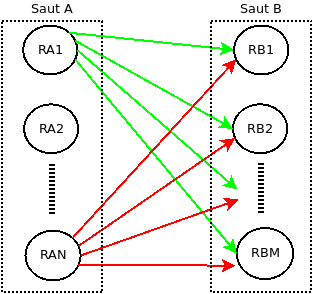
\includegraphics[width=0.5\linewidth]{illustrations/link-inference}
	% Graphic for TeX using PGF
% Title: /home/hayat/RipeAtlasTraceroutesAnalysis/report/illustrations/link-inference.dia
% Creator: Dia v0.97+git
% CreationDate: Thu Nov 29 20:58:09 2018
% For: hayat
% \usepackage{tikz}
% The following commands are not supported in PSTricks at present
% We define them conditionally, so when they are implemented,
% this pgf file will use them.
\ifx\du\undefined
  \newlength{\du}
\fi
\setlength{\du}{15\unitlength}
\begin{tikzpicture}[even odd rule]
\pgftransformxscale{1.000000}
\pgftransformyscale{-1.000000}
\definecolor{dialinecolor}{rgb}{0.000000, 0.000000, 0.000000}
\pgfsetstrokecolor{dialinecolor}
\pgfsetstrokeopacity{1.000000}
\definecolor{diafillcolor}{rgb}{1.000000, 1.000000, 1.000000}
\pgfsetfillcolor{diafillcolor}
\pgfsetfillopacity{1.000000}
\pgfsetlinewidth{0.100000\du}
\pgfsetdash{}{0pt}
\pgfsetmiterjoin
\definecolor{diafillcolor}{rgb}{1.000000, 1.000000, 1.000000}
\pgfsetfillcolor{diafillcolor}
\pgfsetfillopacity{1.000000}
\pgfpathellipse{\pgfpoint{27.430614\du}{13.298442\du}}{\pgfpoint{1.349214\du}{0\du}}{\pgfpoint{0\du}{1.217042\du}}
\pgfusepath{fill}
\definecolor{dialinecolor}{rgb}{0.000000, 0.000000, 0.000000}
\pgfsetstrokecolor{dialinecolor}
\pgfsetstrokeopacity{1.000000}
\pgfpathellipse{\pgfpoint{27.430614\du}{13.298442\du}}{\pgfpoint{1.349214\du}{0\du}}{\pgfpoint{0\du}{1.217042\du}}
\pgfusepath{stroke}
% setfont left to latex
\definecolor{dialinecolor}{rgb}{0.000000, 0.000000, 0.000000}
\pgfsetstrokecolor{dialinecolor}
\pgfsetstrokeopacity{1.000000}
\definecolor{diafillcolor}{rgb}{0.000000, 0.000000, 0.000000}
\pgfsetfillcolor{diafillcolor}
\pgfsetfillopacity{1.000000}
\node[anchor=base,inner sep=0pt, outer sep=0pt,color=dialinecolor] at (27.430614\du,13.493442\du){$R_{1,1}$};
\pgfsetlinewidth{0.100000\du}
\pgfsetdash{}{0pt}
\pgfsetmiterjoin
\definecolor{diafillcolor}{rgb}{1.000000, 1.000000, 1.000000}
\pgfsetfillcolor{diafillcolor}
\pgfsetfillopacity{1.000000}
\pgfpathellipse{\pgfpoint{27.475614\du}{17.238442\du}}{\pgfpoint{1.349214\du}{0\du}}{\pgfpoint{0\du}{1.217042\du}}
\pgfusepath{fill}
\definecolor{dialinecolor}{rgb}{0.000000, 0.000000, 0.000000}
\pgfsetstrokecolor{dialinecolor}
\pgfsetstrokeopacity{1.000000}
\pgfpathellipse{\pgfpoint{27.475614\du}{17.238442\du}}{\pgfpoint{1.349214\du}{0\du}}{\pgfpoint{0\du}{1.217042\du}}
\pgfusepath{stroke}
% setfont left to latex
\definecolor{dialinecolor}{rgb}{0.000000, 0.000000, 0.000000}
\pgfsetstrokecolor{dialinecolor}
\pgfsetstrokeopacity{1.000000}
\definecolor{diafillcolor}{rgb}{0.000000, 0.000000, 0.000000}
\pgfsetfillcolor{diafillcolor}
\pgfsetfillopacity{1.000000}
\node[anchor=base,inner sep=0pt, outer sep=0pt,color=dialinecolor] at (27.475614\du,17.433442\du){$R_{1,2}$};
\pgfsetlinewidth{0.100000\du}
\pgfsetdash{}{0pt}
\pgfsetmiterjoin
\definecolor{diafillcolor}{rgb}{1.000000, 1.000000, 1.000000}
\pgfsetfillcolor{diafillcolor}
\pgfsetfillopacity{1.000000}
\pgfpathellipse{\pgfpoint{27.570578\du}{23.578496\du}}{\pgfpoint{1.376878\du}{0\du}}{\pgfpoint{0\du}{1.241996\du}}
\pgfusepath{fill}
\definecolor{dialinecolor}{rgb}{0.000000, 0.000000, 0.000000}
\pgfsetstrokecolor{dialinecolor}
\pgfsetstrokeopacity{1.000000}
\pgfpathellipse{\pgfpoint{27.570578\du}{23.578496\du}}{\pgfpoint{1.376878\du}{0\du}}{\pgfpoint{0\du}{1.241996\du}}
\pgfusepath{stroke}
% setfont left to latex
\definecolor{dialinecolor}{rgb}{0.000000, 0.000000, 0.000000}
\pgfsetstrokecolor{dialinecolor}
\pgfsetstrokeopacity{1.000000}
\definecolor{diafillcolor}{rgb}{0.000000, 0.000000, 0.000000}
\pgfsetfillcolor{diafillcolor}
\pgfsetfillopacity{1.000000}
\node[anchor=base,inner sep=0pt, outer sep=0pt,color=dialinecolor] at (27.570578\du,23.773496\du){$R_{1,N}$};
\pgfsetlinewidth{0.300000\du}
\pgfsetdash{{\pgflinewidth}{0.200000\du}}{0cm}
\pgfsetbuttcap
{
\definecolor{diafillcolor}{rgb}{0.000000, 0.000000, 0.000000}
\pgfsetfillcolor{diafillcolor}
\pgfsetfillopacity{1.000000}
% was here!!!
\definecolor{dialinecolor}{rgb}{0.000000, 0.000000, 0.000000}
\pgfsetstrokecolor{dialinecolor}
\pgfsetstrokeopacity{1.000000}
\draw (27.540000\du,18.980000\du)--(27.540000\du,21.480000\du);
}
\pgfsetlinewidth{0.100000\du}
\pgfsetdash{}{0pt}
\pgfsetmiterjoin
\definecolor{diafillcolor}{rgb}{1.000000, 1.000000, 1.000000}
\pgfsetfillcolor{diafillcolor}
\pgfsetfillopacity{1.000000}
\pgfpathellipse{\pgfpoint{37.980536\du}{13.298484\du}}{\pgfpoint{1.355136\du}{0\du}}{\pgfpoint{0\du}{1.222384\du}}
\pgfusepath{fill}
\definecolor{dialinecolor}{rgb}{0.000000, 0.000000, 0.000000}
\pgfsetstrokecolor{dialinecolor}
\pgfsetstrokeopacity{1.000000}
\pgfpathellipse{\pgfpoint{37.980536\du}{13.298484\du}}{\pgfpoint{1.355136\du}{0\du}}{\pgfpoint{0\du}{1.222384\du}}
\pgfusepath{stroke}
% setfont left to latex
\definecolor{dialinecolor}{rgb}{0.000000, 0.000000, 0.000000}
\pgfsetstrokecolor{dialinecolor}
\pgfsetstrokeopacity{1.000000}
\definecolor{diafillcolor}{rgb}{0.000000, 0.000000, 0.000000}
\pgfsetfillcolor{diafillcolor}
\pgfsetfillopacity{1.000000}
\node[anchor=base,inner sep=0pt, outer sep=0pt,color=dialinecolor] at (37.980536\du,13.493484\du){$R_{2,1}$};
\pgfsetlinewidth{0.100000\du}
\pgfsetdash{}{0pt}
\pgfsetmiterjoin
\definecolor{diafillcolor}{rgb}{1.000000, 1.000000, 1.000000}
\pgfsetfillcolor{diafillcolor}
\pgfsetfillopacity{1.000000}
\pgfpathellipse{\pgfpoint{37.925536\du}{17.238484\du}}{\pgfpoint{1.355136\du}{0\du}}{\pgfpoint{0\du}{1.222384\du}}
\pgfusepath{fill}
\definecolor{dialinecolor}{rgb}{0.000000, 0.000000, 0.000000}
\pgfsetstrokecolor{dialinecolor}
\pgfsetstrokeopacity{1.000000}
\pgfpathellipse{\pgfpoint{37.925536\du}{17.238484\du}}{\pgfpoint{1.355136\du}{0\du}}{\pgfpoint{0\du}{1.222384\du}}
\pgfusepath{stroke}
% setfont left to latex
\definecolor{dialinecolor}{rgb}{0.000000, 0.000000, 0.000000}
\pgfsetstrokecolor{dialinecolor}
\pgfsetstrokeopacity{1.000000}
\definecolor{diafillcolor}{rgb}{0.000000, 0.000000, 0.000000}
\pgfsetfillcolor{diafillcolor}
\pgfsetfillopacity{1.000000}
\node[anchor=base,inner sep=0pt, outer sep=0pt,color=dialinecolor] at (37.925536\du,17.433484\du){$R_{2,2}$};
\pgfsetlinewidth{0.100000\du}
\pgfsetdash{}{0pt}
\pgfsetmiterjoin
\definecolor{diafillcolor}{rgb}{1.000000, 1.000000, 1.000000}
\pgfsetfillcolor{diafillcolor}
\pgfsetfillopacity{1.000000}
\pgfpathellipse{\pgfpoint{38.170599\du}{23.478445\du}}{\pgfpoint{1.411299\du}{0\du}}{\pgfpoint{0\du}{1.273045\du}}
\pgfusepath{fill}
\definecolor{dialinecolor}{rgb}{0.000000, 0.000000, 0.000000}
\pgfsetstrokecolor{dialinecolor}
\pgfsetstrokeopacity{1.000000}
\pgfpathellipse{\pgfpoint{38.170599\du}{23.478445\du}}{\pgfpoint{1.411299\du}{0\du}}{\pgfpoint{0\du}{1.273045\du}}
\pgfusepath{stroke}
% setfont left to latex
\definecolor{dialinecolor}{rgb}{0.000000, 0.000000, 0.000000}
\pgfsetstrokecolor{dialinecolor}
\pgfsetstrokeopacity{1.000000}
\definecolor{diafillcolor}{rgb}{0.000000, 0.000000, 0.000000}
\pgfsetfillcolor{diafillcolor}
\pgfsetfillopacity{1.000000}
\node[anchor=base,inner sep=0pt, outer sep=0pt,color=dialinecolor] at (38.170599\du,23.673445\du){$R_{1,M}$};
\pgfsetlinewidth{0.300000\du}
\pgfsetdash{{\pgflinewidth}{0.200000\du}}{0cm}
\pgfsetbuttcap
{
\definecolor{diafillcolor}{rgb}{0.000000, 0.000000, 0.000000}
\pgfsetfillcolor{diafillcolor}
\pgfsetfillopacity{1.000000}
% was here!!!
\definecolor{dialinecolor}{rgb}{0.000000, 0.000000, 0.000000}
\pgfsetstrokecolor{dialinecolor}
\pgfsetstrokeopacity{1.000000}
\draw (37.985000\du,18.970000\du)--(37.985000\du,21.470000\du);
}
\pgfsetlinewidth{0.050000\du}
\pgfsetdash{}{0pt}
\pgfsetbuttcap
{
\definecolor{diafillcolor}{rgb}{0.000000, 1.000000, 0.000000}
\pgfsetfillcolor{diafillcolor}
\pgfsetfillopacity{1.000000}
% was here!!!
\pgfsetarrowsstart{stealth}
\definecolor{dialinecolor}{rgb}{0.000000, 1.000000, 0.000000}
\pgfsetstrokecolor{dialinecolor}
\pgfsetstrokeopacity{1.000000}
\draw (28.384600\du,12.437900\du)--(37.022310\du,12.434128\du);
}
\pgfsetlinewidth{0.050000\du}
\pgfsetdash{}{0pt}
\pgfsetbuttcap
{
\definecolor{diafillcolor}{rgb}{1.000000, 0.000000, 0.000000}
\pgfsetfillcolor{diafillcolor}
\pgfsetfillopacity{1.000000}
% was here!!!
\pgfsetarrowsstart{stealth}
\definecolor{dialinecolor}{rgb}{1.000000, 0.000000, 0.000000}
\pgfsetstrokecolor{dialinecolor}
\pgfsetstrokeopacity{1.000000}
\draw (28.842600\du,24.053700\du)--(37.630518\du,24.654584\du);
}
\pgfsetlinewidth{0.100000\du}
\pgfsetdash{{\pgflinewidth}{0.200000\du}}{0cm}
\pgfsetmiterjoin
\pgfsetbuttcap
{\pgfsetcornersarced{\pgfpoint{0.000000\du}{0.000000\du}}\definecolor{dialinecolor}{rgb}{0.000000, 0.000000, 0.000000}
\pgfsetstrokecolor{dialinecolor}
\pgfsetstrokeopacity{1.000000}
\draw (25.638764\du,11.830038\du)--(25.638764\du,25.156536\du)--(29.721269\du,25.156536\du)--(29.721269\du,11.830038\du)--cycle;
}\pgfsetlinewidth{0.100000\du}
\pgfsetdash{{\pgflinewidth}{0.200000\du}}{0cm}
\pgfsetmiterjoin
\pgfsetbuttcap
{\pgfsetcornersarced{\pgfpoint{0.000000\du}{0.000000\du}}\definecolor{dialinecolor}{rgb}{0.000000, 0.000000, 0.000000}
\pgfsetstrokecolor{dialinecolor}
\pgfsetstrokeopacity{1.000000}
\draw (36.096688\du,11.857262\du)--(36.096688\du,25.128574\du)--(39.871607\du,25.128574\du)--(39.871607\du,11.857262\du)--cycle;
}% setfont left to latex
\definecolor{dialinecolor}{rgb}{0.000000, 0.000000, 0.000000}
\pgfsetstrokecolor{dialinecolor}
\pgfsetstrokeopacity{1.000000}
\definecolor{diafillcolor}{rgb}{0.000000, 0.000000, 0.000000}
\pgfsetfillcolor{diafillcolor}
\pgfsetfillopacity{1.000000}
\node[anchor=base west,inner sep=0pt,outer sep=0pt,color=dialinecolor] at (26.470600\du,11.464400\du){$ h_1 $};
% setfont left to latex
\definecolor{dialinecolor}{rgb}{0.000000, 0.000000, 0.000000}
\pgfsetstrokecolor{dialinecolor}
\pgfsetstrokeopacity{1.000000}
\definecolor{diafillcolor}{rgb}{0.000000, 0.000000, 0.000000}
\pgfsetfillcolor{diafillcolor}
\pgfsetfillopacity{1.000000}
\node[anchor=base west,inner sep=0pt,outer sep=0pt,color=dialinecolor] at (36.898700\du,11.464100\du){$ h_2 $};
\pgfsetlinewidth{0.050000\du}
\pgfsetdash{}{0pt}
\pgfsetbuttcap
{
\definecolor{diafillcolor}{rgb}{0.000000, 0.000000, 1.000000}
\pgfsetfillcolor{diafillcolor}
\pgfsetfillopacity{1.000000}
% was here!!!
\pgfsetarrowsstart{stealth}
\definecolor{dialinecolor}{rgb}{0.000000, 0.000000, 1.000000}
\pgfsetstrokecolor{dialinecolor}
\pgfsetstrokeopacity{1.000000}
\draw (28.779828\du,13.298442\du)--(37.406948\du,16.109148\du);
}
\pgfsetlinewidth{0.050000\du}
\pgfsetdash{}{0pt}
\pgfsetbuttcap
{
\definecolor{diafillcolor}{rgb}{0.000000, 1.000000, 0.000000}
\pgfsetfillcolor{diafillcolor}
\pgfsetfillopacity{1.000000}
% was here!!!
\pgfsetarrowsstart{stealth}
\definecolor{dialinecolor}{rgb}{0.000000, 1.000000, 0.000000}
\pgfsetstrokecolor{dialinecolor}
\pgfsetstrokeopacity{1.000000}
\draw (28.722125\du,16.772700\du)--(36.728554\du,12.830698\du);
}
\pgfsetlinewidth{0.050000\du}
\pgfsetdash{}{0pt}
\pgfsetbuttcap
{
\definecolor{diafillcolor}{rgb}{0.000000, 1.000000, 0.000000}
\pgfsetfillcolor{diafillcolor}
\pgfsetfillopacity{1.000000}
% was here!!!
\pgfsetarrowsstart{stealth}
\definecolor{dialinecolor}{rgb}{0.000000, 1.000000, 0.000000}
\pgfsetstrokecolor{dialinecolor}
\pgfsetstrokeopacity{1.000000}
\draw (28.602774\du,20.095348\du)--(36.625400\du,13.298484\du);
}
\pgfsetlinewidth{0.050000\du}
\pgfsetdash{}{0pt}
\pgfsetbuttcap
{
\definecolor{diafillcolor}{rgb}{0.000000, 1.000000, 0.000000}
\pgfsetfillcolor{diafillcolor}
\pgfsetfillopacity{1.000000}
% was here!!!
\pgfsetarrowsstart{stealth}
\definecolor{dialinecolor}{rgb}{0.000000, 1.000000, 0.000000}
\pgfsetstrokecolor{dialinecolor}
\pgfsetstrokeopacity{1.000000}
\draw (28.097487\du,22.431041\du)--(36.728554\du,13.766270\du);
}
\pgfsetlinewidth{0.050000\du}
\pgfsetdash{}{0pt}
\pgfsetbuttcap
{
\definecolor{diafillcolor}{rgb}{0.000000, 0.000000, 1.000000}
\pgfsetfillcolor{diafillcolor}
\pgfsetfillopacity{1.000000}
% was here!!!
\pgfsetarrowsstart{stealth}
\definecolor{dialinecolor}{rgb}{0.000000, 0.000000, 1.000000}
\pgfsetstrokecolor{dialinecolor}
\pgfsetstrokeopacity{1.000000}
\draw (28.824828\du,17.238442\du)--(36.967310\du,16.374128\du);
}
\pgfsetlinewidth{0.050000\du}
\pgfsetdash{}{0pt}
\pgfsetbuttcap
{
\definecolor{diafillcolor}{rgb}{0.000000, 0.000000, 1.000000}
\pgfsetfillcolor{diafillcolor}
\pgfsetfillopacity{1.000000}
% was here!!!
\pgfsetarrowsstart{stealth}
\definecolor{dialinecolor}{rgb}{0.000000, 0.000000, 1.000000}
\pgfsetstrokecolor{dialinecolor}
\pgfsetstrokeopacity{1.000000}
\draw (28.798511\du,20.486821\du)--(36.673554\du,16.770698\du);
}
\pgfsetlinewidth{0.050000\du}
\pgfsetdash{}{0pt}
\pgfsetbuttcap
{
\definecolor{diafillcolor}{rgb}{0.000000, 0.000000, 1.000000}
\pgfsetfillcolor{diafillcolor}
\pgfsetfillopacity{1.000000}
% was here!!!
\pgfsetarrowsstart{stealth}
\definecolor{dialinecolor}{rgb}{0.000000, 0.000000, 1.000000}
\pgfsetstrokecolor{dialinecolor}
\pgfsetstrokeopacity{1.000000}
\draw (28.544178\du,22.700272\du)--(36.516123\du,17.355037\du);
}
\pgfsetlinewidth{0.050000\du}
\pgfsetdash{}{0pt}
\pgfsetbuttcap
{
\definecolor{diafillcolor}{rgb}{1.000000, 0.000000, 0.000000}
\pgfsetfillcolor{diafillcolor}
\pgfsetfillopacity{1.000000}
% was here!!!
\pgfsetarrowsstart{stealth}
\definecolor{dialinecolor}{rgb}{1.000000, 0.000000, 0.000000}
\pgfsetstrokecolor{dialinecolor}
\pgfsetstrokeopacity{1.000000}
\draw (28.938323\du,20.850332\du)--(36.866729\du,23.965618\du);
}
\pgfsetlinewidth{0.050000\du}
\pgfsetdash{}{0pt}
\pgfsetbuttcap
{
\definecolor{diafillcolor}{rgb}{1.000000, 0.000000, 0.000000}
\pgfsetfillcolor{diafillcolor}
\pgfsetfillopacity{1.000000}
% was here!!!
\pgfsetarrowsstart{stealth}
\definecolor{dialinecolor}{rgb}{1.000000, 0.000000, 0.000000}
\pgfsetstrokecolor{dialinecolor}
\pgfsetstrokeopacity{1.000000}
\draw (28.722125\du,17.704183\du)--(36.712688\du,23.381227\du);
}
\pgfsetlinewidth{0.050000\du}
\pgfsetdash{}{0pt}
\pgfsetbuttcap
{
\definecolor{diafillcolor}{rgb}{1.000000, 0.000000, 0.000000}
\pgfsetfillcolor{diafillcolor}
\pgfsetfillopacity{1.000000}
% was here!!!
\pgfsetarrowsstart{stealth}
\definecolor{dialinecolor}{rgb}{1.000000, 0.000000, 0.000000}
\pgfsetstrokecolor{dialinecolor}
\pgfsetstrokeopacity{1.000000}
\draw (28.677125\du,13.764183\du)--(36.866729\du,22.991272\du);
}
\end{tikzpicture}

}
	\caption{Inférence des liens possibles entre les routeurs des deux sauts consécutifs $R_{a,i}$ et $R_{b,j}$}
	\label{fig:link-inference}
\end{figure}
\paragraph{5. Caractérisation des liens} avec leurs RTTs différentiels. A cette étape, on calcule le RTT différentiel de chaque  lien, au sein d'un traceroute donné, en calculant la différence entre les RTTs des deux routeurs impliqués dans le  lien en question. En plus du RTT différentiel, on note aussi la sonde Atlas ayant effectué la requête traceroute où le lien a été identifié. 

\paragraph{6. Fusion des informations d'un lien} Etant donné qu'un lien (IP1, IP2) peut être identifié plusieurs fois pendant une même période $d_k$ d'une part, et le lien (IP2, IP1) est similaire au lien  (IP1, IP2) d'autre part, la fusion permet de construire une nouvelle distribution des RTTs différentiels caractérisant le lien (IP1, IP2) qui reprend les RTTs différentiels du lien (IP1, IP2) ainsi que ceux du lien (IP2, IP1).

Dans le travail de référence, la similarité de deux liens  implique que les RTTs différentiels qui caractérisent un lien (IP2, IP1) caractérisent aussi le lien (IP1, IP2); ces deux lien partagent les même routeurs.


A la fin de l'étape 6, tous les traceroutes sont préparés. A présent, l'objectif est d'identifier les dates pendant lesquelles des anomalies ont été détectées. Pour ce faire, l'idée du travail de référence est de conserver, pour un lien donné, une référence du RTT différentiel médian.  Cette référence est d'abord comparée avec la médiane courante des RTTs différentiels,  puis,  mise à jour au fur et à mesure   tout au long de la période de l'analyse.

  
  \paragraph{7. Calcul de la médiane des RTTs différentiels et   l'intervalle de confiance courant} du lien analysé. Pour un lien donné, on calcule la médiane des RTTs différentiels d'une $d_k$, ensuite on calcule les deux bornes de l'intervalle de confiance courant pour ce $d_k$.  
  
 
  
  \paragraph{8. Mise à jour de la médiane et de l'intervalle  de confiance de  référence du lien analysé.} La médiane des RTTs différentiels de référence ainsi que l'intervalle de confiance de référence sont mise à jour tant que la période déclenchant la détection des anomalies n'est pas atteinte.  La mise à jour de la référence : médiane et les bornes de l'intervalle de confiance se base sur la moyenne mobile exponentielle . Cette méthode prend en compte les valeurs antérieures ainsi que celles récentes en étant dirigée par le paramètre \textit{confInterval} décrit dans la section \ref{par:parametre-de-lanalyse}.
  

 \paragraph{9. Comparaison des intervalles de confiance} 

La comparaison de l'état courant du lien avec celui de référence est effectuée en analysant le chevauchement d'intervalles de confiance  courant et de référence. Le délai d'un lien est jugé normal si son intervalle de confiance courant est inclus dans l'intervalle de confiance de référence. C'est le cas $1$ dans la Figure 	\ref{fig:intervals-comparaison},  \textit{referenceLow} et \textit{referenceHight} sont les bornes de l'intervalle de confiance de référence.  \textit{currentLow} et \textit{currentHight} sont les bornes de l'intervalle de confiance courant.

D'après le travail de référence, on distingue quatre cas possibles  illustrés dans la Figure 	\ref{fig:intervals-comparaison}:

\textbf{Cas 1 :} le délai du lien est normal.

\textbf{Cas 2 :} le délai du lien est anormal.

\textbf{Cas 3 :} le délai du lien est anormal.

\textbf{Cas 4 :} le délai du lien est anormal.

Dans le cas où le délai est jugé anormal, on introduit ce qu'on appelle la \textit{déviation}. Cette métrique caractérise l'anomalie détectée. Elle est calculée différemment dans le cas où le délai est anormal.

\begin{figure}[H]
	\centering
	\captionsetup{justification=centering}
	\resizebox{\textwidth}{!}{
		% Graphic for TeX using PGF
% Title: /home/hayat/RipeAtlasTraceroutesAnalysis/report/illustrations/intervals-comparaison.dia
% Creator: Dia v0.97+git
% CreationDate: Tue Dec  4 13:30:20 2018
% For: hayat
% \usepackage{tikz}
% The following commands are not supported in PSTricks at present
% We define them conditionally, so when they are implemented,
% this pgf file will use them.
\ifx\du\undefined
  \newlength{\du}
\fi
\setlength{\du}{15\unitlength}
\begin{tikzpicture}[even odd rule]
\pgftransformxscale{1.000000}
\pgftransformyscale{-1.000000}
\definecolor{dialinecolor}{rgb}{0.000000, 0.000000, 0.000000}
\pgfsetstrokecolor{dialinecolor}
\pgfsetstrokeopacity{1.000000}
\definecolor{diafillcolor}{rgb}{1.000000, 1.000000, 1.000000}
\pgfsetfillcolor{diafillcolor}
\pgfsetfillopacity{1.000000}
\pgfsetlinewidth{0.100000\du}
\pgfsetdash{}{0pt}
\pgfsetbuttcap
{
\definecolor{diafillcolor}{rgb}{0.662745, 0.709804, 0.674510}
\pgfsetfillcolor{diafillcolor}
\pgfsetfillopacity{1.000000}
% was here!!!
}
\definecolor{dialinecolor}{rgb}{0.662745, 0.709804, 0.674510}
\pgfsetstrokecolor{dialinecolor}
\pgfsetstrokeopacity{1.000000}
\draw (14.150000\du,0.400000\du)--(27.000000\du,0.400000\du);
\pgfsetlinewidth{0.100000\du}
\pgfsetdash{}{0pt}
\pgfsetmiterjoin
\pgfsetbuttcap
\definecolor{diafillcolor}{rgb}{0.662745, 0.709804, 0.674510}
\pgfsetfillcolor{diafillcolor}
\pgfsetfillopacity{1.000000}
\fill (13.900000\du,0.550000\du)--(13.900000\du,0.250000\du)--(14.200000\du,0.250000\du)--(14.200000\du,0.550000\du)--cycle;
\definecolor{dialinecolor}{rgb}{0.662745, 0.709804, 0.674510}
\pgfsetstrokecolor{dialinecolor}
\pgfsetstrokeopacity{1.000000}
\draw (14.050000\du,0.700000\du)--(14.050000\du,0.100000\du);
\pgfsetlinewidth{0.100000\du}
\pgfsetdash{}{0pt}
\pgfsetmiterjoin
\pgfsetbuttcap
\definecolor{diafillcolor}{rgb}{0.662745, 0.709804, 0.674510}
\pgfsetfillcolor{diafillcolor}
\pgfsetfillopacity{1.000000}
\fill (27.250000\du,0.250000\du)--(27.250000\du,0.550000\du)--(26.950000\du,0.550000\du)--(26.950000\du,0.250000\du)--cycle;
\definecolor{dialinecolor}{rgb}{0.662745, 0.709804, 0.674510}
\pgfsetstrokecolor{dialinecolor}
\pgfsetstrokeopacity{1.000000}
\draw (27.100000\du,0.100000\du)--(27.100000\du,0.700000\du);
\pgfsetlinewidth{0.100000\du}
\pgfsetdash{}{0pt}
\pgfsetbuttcap
{
\definecolor{diafillcolor}{rgb}{0.000000, 0.000000, 0.000000}
\pgfsetfillcolor{diafillcolor}
\pgfsetfillopacity{1.000000}
% was here!!!
}
\definecolor{dialinecolor}{rgb}{0.000000, 0.000000, 0.000000}
\pgfsetstrokecolor{dialinecolor}
\pgfsetstrokeopacity{1.000000}
\draw (16.150000\du,2.450000\du)--(24.800000\du,2.450000\du);
\pgfsetlinewidth{0.100000\du}
\pgfsetdash{}{0pt}
\pgfsetmiterjoin
\pgfsetbuttcap
\definecolor{diafillcolor}{rgb}{0.000000, 0.000000, 0.000000}
\pgfsetfillcolor{diafillcolor}
\pgfsetfillopacity{1.000000}
\fill (15.900000\du,2.600000\du)--(15.900000\du,2.300000\du)--(16.200000\du,2.300000\du)--(16.200000\du,2.600000\du)--cycle;
\definecolor{dialinecolor}{rgb}{0.000000, 0.000000, 0.000000}
\pgfsetstrokecolor{dialinecolor}
\pgfsetstrokeopacity{1.000000}
\draw (16.050000\du,2.750000\du)--(16.050000\du,2.150000\du);
\pgfsetlinewidth{0.100000\du}
\pgfsetdash{}{0pt}
\pgfsetmiterjoin
\pgfsetbuttcap
\definecolor{diafillcolor}{rgb}{0.000000, 0.000000, 0.000000}
\pgfsetfillcolor{diafillcolor}
\pgfsetfillopacity{1.000000}
\fill (25.050000\du,2.300000\du)--(25.050000\du,2.600000\du)--(24.750000\du,2.600000\du)--(24.750000\du,2.300000\du)--cycle;
\definecolor{dialinecolor}{rgb}{0.000000, 0.000000, 0.000000}
\pgfsetstrokecolor{dialinecolor}
\pgfsetstrokeopacity{1.000000}
\draw (24.900000\du,2.150000\du)--(24.900000\du,2.750000\du);
\pgfsetlinewidth{0.100000\du}
\pgfsetdash{}{0pt}
\pgfsetbuttcap
{
\definecolor{diafillcolor}{rgb}{0.662745, 0.709804, 0.674510}
\pgfsetfillcolor{diafillcolor}
\pgfsetfillopacity{1.000000}
% was here!!!
}
\definecolor{dialinecolor}{rgb}{0.662745, 0.709804, 0.674510}
\pgfsetstrokecolor{dialinecolor}
\pgfsetstrokeopacity{1.000000}
\draw (14.008246\du,11.548114\du)--(26.858246\du,11.548114\du);
\pgfsetlinewidth{0.100000\du}
\pgfsetdash{}{0pt}
\pgfsetmiterjoin
\pgfsetbuttcap
\definecolor{diafillcolor}{rgb}{0.662745, 0.709804, 0.674510}
\pgfsetfillcolor{diafillcolor}
\pgfsetfillopacity{1.000000}
\fill (13.758246\du,11.698114\du)--(13.758246\du,11.398114\du)--(14.058246\du,11.398114\du)--(14.058246\du,11.698114\du)--cycle;
\definecolor{dialinecolor}{rgb}{0.662745, 0.709804, 0.674510}
\pgfsetstrokecolor{dialinecolor}
\pgfsetstrokeopacity{1.000000}
\draw (13.908246\du,11.848114\du)--(13.908246\du,11.248114\du);
\pgfsetlinewidth{0.100000\du}
\pgfsetdash{}{0pt}
\pgfsetmiterjoin
\pgfsetbuttcap
\definecolor{diafillcolor}{rgb}{0.662745, 0.709804, 0.674510}
\pgfsetfillcolor{diafillcolor}
\pgfsetfillopacity{1.000000}
\fill (27.108246\du,11.398114\du)--(27.108246\du,11.698114\du)--(26.808246\du,11.698114\du)--(26.808246\du,11.398114\du)--cycle;
\definecolor{dialinecolor}{rgb}{0.662745, 0.709804, 0.674510}
\pgfsetstrokecolor{dialinecolor}
\pgfsetstrokeopacity{1.000000}
\draw (26.958246\du,11.248114\du)--(26.958246\du,11.848114\du);
\pgfsetlinewidth{0.100000\du}
\pgfsetdash{}{0pt}
\pgfsetbuttcap
{
\definecolor{diafillcolor}{rgb}{0.000000, 0.000000, 0.000000}
\pgfsetfillcolor{diafillcolor}
\pgfsetfillopacity{1.000000}
% was here!!!
}
\definecolor{dialinecolor}{rgb}{0.000000, 0.000000, 0.000000}
\pgfsetstrokecolor{dialinecolor}
\pgfsetstrokeopacity{1.000000}
\draw (23.108246\du,13.598114\du)--(31.758246\du,13.598114\du);
\pgfsetlinewidth{0.100000\du}
\pgfsetdash{}{0pt}
\pgfsetmiterjoin
\pgfsetbuttcap
\definecolor{diafillcolor}{rgb}{0.000000, 0.000000, 0.000000}
\pgfsetfillcolor{diafillcolor}
\pgfsetfillopacity{1.000000}
\fill (22.858246\du,13.748114\du)--(22.858246\du,13.448114\du)--(23.158246\du,13.448114\du)--(23.158246\du,13.748114\du)--cycle;
\definecolor{dialinecolor}{rgb}{0.000000, 0.000000, 0.000000}
\pgfsetstrokecolor{dialinecolor}
\pgfsetstrokeopacity{1.000000}
\draw (23.008246\du,13.898114\du)--(23.008246\du,13.298114\du);
\pgfsetlinewidth{0.100000\du}
\pgfsetdash{}{0pt}
\pgfsetmiterjoin
\pgfsetbuttcap
\definecolor{diafillcolor}{rgb}{0.000000, 0.000000, 0.000000}
\pgfsetfillcolor{diafillcolor}
\pgfsetfillopacity{1.000000}
\fill (32.008246\du,13.448114\du)--(32.008246\du,13.748114\du)--(31.708246\du,13.748114\du)--(31.708246\du,13.448114\du)--cycle;
\definecolor{dialinecolor}{rgb}{0.000000, 0.000000, 0.000000}
\pgfsetstrokecolor{dialinecolor}
\pgfsetstrokeopacity{1.000000}
\draw (31.858246\du,13.298114\du)--(31.858246\du,13.898114\du);
\pgfsetlinewidth{0.100000\du}
\pgfsetdash{}{0pt}
\pgfsetbuttcap
{
\definecolor{diafillcolor}{rgb}{0.662745, 0.709804, 0.674510}
\pgfsetfillcolor{diafillcolor}
\pgfsetfillopacity{1.000000}
% was here!!!
}
\definecolor{dialinecolor}{rgb}{0.662745, 0.709804, 0.674510}
\pgfsetstrokecolor{dialinecolor}
\pgfsetstrokeopacity{1.000000}
\draw (14.108246\du,17.048114\du)--(26.958246\du,17.048114\du);
\pgfsetlinewidth{0.100000\du}
\pgfsetdash{}{0pt}
\pgfsetmiterjoin
\pgfsetbuttcap
\definecolor{diafillcolor}{rgb}{0.662745, 0.709804, 0.674510}
\pgfsetfillcolor{diafillcolor}
\pgfsetfillopacity{1.000000}
\fill (13.858246\du,17.198114\du)--(13.858246\du,16.898114\du)--(14.158246\du,16.898114\du)--(14.158246\du,17.198114\du)--cycle;
\definecolor{dialinecolor}{rgb}{0.662745, 0.709804, 0.674510}
\pgfsetstrokecolor{dialinecolor}
\pgfsetstrokeopacity{1.000000}
\draw (14.008246\du,17.348114\du)--(14.008246\du,16.748114\du);
\pgfsetlinewidth{0.100000\du}
\pgfsetdash{}{0pt}
\pgfsetmiterjoin
\pgfsetbuttcap
\definecolor{diafillcolor}{rgb}{0.662745, 0.709804, 0.674510}
\pgfsetfillcolor{diafillcolor}
\pgfsetfillopacity{1.000000}
\fill (27.208246\du,16.898114\du)--(27.208246\du,17.198114\du)--(26.908246\du,17.198114\du)--(26.908246\du,16.898114\du)--cycle;
\definecolor{dialinecolor}{rgb}{0.662745, 0.709804, 0.674510}
\pgfsetstrokecolor{dialinecolor}
\pgfsetstrokeopacity{1.000000}
\draw (27.058246\du,16.748114\du)--(27.058246\du,17.348114\du);
\pgfsetlinewidth{0.100000\du}
\pgfsetdash{}{0pt}
\pgfsetbuttcap
{
\definecolor{diafillcolor}{rgb}{0.000000, 0.000000, 0.000000}
\pgfsetfillcolor{diafillcolor}
\pgfsetfillopacity{1.000000}
% was here!!!
}
\definecolor{dialinecolor}{rgb}{0.000000, 0.000000, 0.000000}
\pgfsetstrokecolor{dialinecolor}
\pgfsetstrokeopacity{1.000000}
\draw (9.308246\du,19.048114\du)--(17.958246\du,19.048114\du);
\pgfsetlinewidth{0.100000\du}
\pgfsetdash{}{0pt}
\pgfsetmiterjoin
\pgfsetbuttcap
\definecolor{diafillcolor}{rgb}{0.000000, 0.000000, 0.000000}
\pgfsetfillcolor{diafillcolor}
\pgfsetfillopacity{1.000000}
\fill (9.058246\du,19.198114\du)--(9.058246\du,18.898114\du)--(9.358246\du,18.898114\du)--(9.358246\du,19.198114\du)--cycle;
\definecolor{dialinecolor}{rgb}{0.000000, 0.000000, 0.000000}
\pgfsetstrokecolor{dialinecolor}
\pgfsetstrokeopacity{1.000000}
\draw (9.208246\du,19.348114\du)--(9.208246\du,18.748114\du);
\pgfsetlinewidth{0.100000\du}
\pgfsetdash{}{0pt}
\pgfsetmiterjoin
\pgfsetbuttcap
\definecolor{diafillcolor}{rgb}{0.000000, 0.000000, 0.000000}
\pgfsetfillcolor{diafillcolor}
\pgfsetfillopacity{1.000000}
\fill (18.208246\du,18.898114\du)--(18.208246\du,19.198114\du)--(17.908246\du,19.198114\du)--(17.908246\du,18.898114\du)--cycle;
\definecolor{dialinecolor}{rgb}{0.000000, 0.000000, 0.000000}
\pgfsetstrokecolor{dialinecolor}
\pgfsetstrokeopacity{1.000000}
\draw (18.058246\du,18.748114\du)--(18.058246\du,19.348114\du);
\pgfsetlinewidth{0.100000\du}
\pgfsetdash{{\pgflinewidth}{0.200000\du}}{0cm}
\pgfsetbuttcap
{
\definecolor{diafillcolor}{rgb}{0.000000, 0.000000, 0.000000}
\pgfsetfillcolor{diafillcolor}
\pgfsetfillopacity{1.000000}
% was here!!!
\pgfsetarrowsend{stealth}
\definecolor{dialinecolor}{rgb}{0.000000, 0.000000, 0.000000}
\pgfsetstrokecolor{dialinecolor}
\pgfsetstrokeopacity{1.000000}
\draw (5.050000\du,21.000000\du)--(38.800000\du,20.950000\du);
}
\pgfsetlinewidth{0.100000\du}
\pgfsetdash{}{0pt}
\pgfsetbuttcap
{
\definecolor{diafillcolor}{rgb}{0.662745, 0.709804, 0.674510}
\pgfsetfillcolor{diafillcolor}
\pgfsetfillopacity{1.000000}
% was here!!!
}
\definecolor{dialinecolor}{rgb}{0.662745, 0.709804, 0.674510}
\pgfsetstrokecolor{dialinecolor}
\pgfsetstrokeopacity{1.000000}
\draw (13.958246\du,6.048114\du)--(26.808246\du,6.048114\du);
\pgfsetlinewidth{0.100000\du}
\pgfsetdash{}{0pt}
\pgfsetmiterjoin
\pgfsetbuttcap
\definecolor{diafillcolor}{rgb}{0.662745, 0.709804, 0.674510}
\pgfsetfillcolor{diafillcolor}
\pgfsetfillopacity{1.000000}
\fill (13.708246\du,6.198114\du)--(13.708246\du,5.898114\du)--(14.008246\du,5.898114\du)--(14.008246\du,6.198114\du)--cycle;
\definecolor{dialinecolor}{rgb}{0.662745, 0.709804, 0.674510}
\pgfsetstrokecolor{dialinecolor}
\pgfsetstrokeopacity{1.000000}
\draw (13.858246\du,6.348114\du)--(13.858246\du,5.748114\du);
\pgfsetlinewidth{0.100000\du}
\pgfsetdash{}{0pt}
\pgfsetmiterjoin
\pgfsetbuttcap
\definecolor{diafillcolor}{rgb}{0.662745, 0.709804, 0.674510}
\pgfsetfillcolor{diafillcolor}
\pgfsetfillopacity{1.000000}
\fill (27.058246\du,5.898114\du)--(27.058246\du,6.198114\du)--(26.758246\du,6.198114\du)--(26.758246\du,5.898114\du)--cycle;
\definecolor{dialinecolor}{rgb}{0.662745, 0.709804, 0.674510}
\pgfsetstrokecolor{dialinecolor}
\pgfsetstrokeopacity{1.000000}
\draw (26.908246\du,5.748114\du)--(26.908246\du,6.348114\du);
\pgfsetlinewidth{0.100000\du}
\pgfsetdash{}{0pt}
\pgfsetbuttcap
{
\definecolor{diafillcolor}{rgb}{0.000000, 0.000000, 0.000000}
\pgfsetfillcolor{diafillcolor}
\pgfsetfillopacity{1.000000}
% was here!!!
}
\definecolor{dialinecolor}{rgb}{0.000000, 0.000000, 0.000000}
\pgfsetstrokecolor{dialinecolor}
\pgfsetstrokeopacity{1.000000}
\draw (10.049999\du,8.049461\du)--(32.750001\du,8.000539\du);
\pgfsetlinewidth{0.100000\du}
\pgfsetdash{}{0pt}
\pgfsetmiterjoin
\pgfsetbuttcap
\definecolor{diafillcolor}{rgb}{0.000000, 0.000000, 0.000000}
\pgfsetfillcolor{diafillcolor}
\pgfsetfillopacity{1.000000}
\fill (9.800323\du,8.200000\du)--(9.799677\du,7.900000\du)--(10.099676\du,7.899354\du)--(10.100323\du,8.199353\du)--cycle;
\definecolor{dialinecolor}{rgb}{0.000000, 0.000000, 0.000000}
\pgfsetstrokecolor{dialinecolor}
\pgfsetstrokeopacity{1.000000}
\draw (9.950646\du,8.349676\du)--(9.949353\du,7.749677\du);
\pgfsetlinewidth{0.100000\du}
\pgfsetdash{}{0pt}
\pgfsetmiterjoin
\pgfsetbuttcap
\definecolor{diafillcolor}{rgb}{0.000000, 0.000000, 0.000000}
\pgfsetfillcolor{diafillcolor}
\pgfsetfillopacity{1.000000}
\fill (32.999677\du,7.850000\du)--(33.000323\du,8.150000\du)--(32.700324\du,8.150646\du)--(32.699677\du,7.850647\du)--cycle;
\definecolor{dialinecolor}{rgb}{0.000000, 0.000000, 0.000000}
\pgfsetstrokecolor{dialinecolor}
\pgfsetstrokeopacity{1.000000}
\draw (32.849354\du,7.700324\du)--(32.850647\du,8.300323\du);
\pgfsetlinewidth{0.050000\du}
\pgfsetdash{}{0pt}
\pgfsetmiterjoin
\pgfsetbuttcap
{\pgfsetcornersarced{\pgfpoint{0.000000\du}{0.000000\du}}\definecolor{dialinecolor}{rgb}{0.000000, 0.000000, 0.000000}
\pgfsetstrokecolor{dialinecolor}
\pgfsetstrokeopacity{1.000000}
\draw (6.900000\du,4.500000\du)--(6.900000\du,8.950000\du)--(36.950000\du,8.950000\du)--(36.950000\du,4.500000\du)--cycle;
}% setfont left to latex
\definecolor{dialinecolor}{rgb}{0.000000, 0.000000, 0.000000}
\pgfsetstrokecolor{dialinecolor}
\pgfsetstrokeopacity{1.000000}
\definecolor{diafillcolor}{rgb}{0.000000, 0.000000, 0.000000}
\pgfsetfillcolor{diafillcolor}
\pgfsetfillopacity{1.000000}
\node[anchor=base west,inner sep=0pt,outer sep=0pt,color=dialinecolor] at (7.950000\du,7.550000\du){currentLow};
% setfont left to latex
\definecolor{dialinecolor}{rgb}{0.000000, 0.000000, 0.000000}
\pgfsetstrokecolor{dialinecolor}
\pgfsetstrokeopacity{1.000000}
\definecolor{diafillcolor}{rgb}{0.000000, 0.000000, 0.000000}
\pgfsetfillcolor{diafillcolor}
\pgfsetfillopacity{1.000000}
\node[anchor=base west,inner sep=0pt,outer sep=0pt,color=dialinecolor] at (30.800000\du,7.500000\du){currentHight};
% setfont left to latex
\definecolor{dialinecolor}{rgb}{0.282353, 0.313726, 0.290196}
\pgfsetstrokecolor{dialinecolor}
\pgfsetstrokeopacity{1.000000}
\definecolor{diafillcolor}{rgb}{0.282353, 0.313726, 0.290196}
\pgfsetfillcolor{diafillcolor}
\pgfsetfillopacity{1.000000}
\node[anchor=base west,inner sep=0pt,outer sep=0pt,color=dialinecolor] at (11.450000\du,5.550000\du){referenceLow};
% setfont left to latex
\definecolor{dialinecolor}{rgb}{0.282353, 0.313726, 0.290196}
\pgfsetstrokecolor{dialinecolor}
\pgfsetstrokeopacity{1.000000}
\definecolor{diafillcolor}{rgb}{0.282353, 0.313726, 0.290196}
\pgfsetfillcolor{diafillcolor}
\pgfsetfillopacity{1.000000}
\node[anchor=base west,inner sep=0pt,outer sep=0pt,color=dialinecolor] at (23.750000\du,5.550000\du){referenceHight};
% setfont left to latex
\definecolor{dialinecolor}{rgb}{0.282353, 0.313726, 0.290196}
\pgfsetstrokecolor{dialinecolor}
\pgfsetstrokeopacity{1.000000}
\definecolor{diafillcolor}{rgb}{0.282353, 0.313726, 0.290196}
\pgfsetfillcolor{diafillcolor}
\pgfsetfillopacity{1.000000}
\node[anchor=base west,inner sep=0pt,outer sep=0pt,color=dialinecolor] at (24.545000\du,-0.297500\du){referenceHight};
% setfont left to latex
\definecolor{dialinecolor}{rgb}{0.282353, 0.313726, 0.290196}
\pgfsetstrokecolor{dialinecolor}
\pgfsetstrokeopacity{1.000000}
\definecolor{diafillcolor}{rgb}{0.282353, 0.313726, 0.290196}
\pgfsetfillcolor{diafillcolor}
\pgfsetfillopacity{1.000000}
\node[anchor=base west,inner sep=0pt,outer sep=0pt,color=dialinecolor] at (24.390000\du,10.792500\du){referenceHight};
% setfont left to latex
\definecolor{dialinecolor}{rgb}{0.282353, 0.313726, 0.290196}
\pgfsetstrokecolor{dialinecolor}
\pgfsetstrokeopacity{1.000000}
\definecolor{diafillcolor}{rgb}{0.282353, 0.313726, 0.290196}
\pgfsetfillcolor{diafillcolor}
\pgfsetfillopacity{1.000000}
\node[anchor=base west,inner sep=0pt,outer sep=0pt,color=dialinecolor] at (24.485000\du,16.282500\du){referenceHight};
% setfont left to latex
\definecolor{dialinecolor}{rgb}{0.282353, 0.313726, 0.290196}
\pgfsetstrokecolor{dialinecolor}
\pgfsetstrokeopacity{1.000000}
\definecolor{diafillcolor}{rgb}{0.282353, 0.313726, 0.290196}
\pgfsetfillcolor{diafillcolor}
\pgfsetfillopacity{1.000000}
\node[anchor=base west,inner sep=0pt,outer sep=0pt,color=dialinecolor] at (12.045000\du,-0.247500\du){referenceLow};
% setfont left to latex
\definecolor{dialinecolor}{rgb}{0.282353, 0.313726, 0.290196}
\pgfsetstrokecolor{dialinecolor}
\pgfsetstrokeopacity{1.000000}
\definecolor{diafillcolor}{rgb}{0.282353, 0.313726, 0.290196}
\pgfsetfillcolor{diafillcolor}
\pgfsetfillopacity{1.000000}
\node[anchor=base west,inner sep=0pt,outer sep=0pt,color=dialinecolor] at (11.340000\du,10.892500\du){referenceLow};
% setfont left to latex
\definecolor{dialinecolor}{rgb}{0.282353, 0.313726, 0.290196}
\pgfsetstrokecolor{dialinecolor}
\pgfsetstrokeopacity{1.000000}
\definecolor{diafillcolor}{rgb}{0.282353, 0.313726, 0.290196}
\pgfsetfillcolor{diafillcolor}
\pgfsetfillopacity{1.000000}
\node[anchor=base west,inner sep=0pt,outer sep=0pt,color=dialinecolor] at (11.535000\du,16.532500\du){referenceLow};
% setfont left to latex
\definecolor{dialinecolor}{rgb}{0.000000, 0.000000, 0.000000}
\pgfsetstrokecolor{dialinecolor}
\pgfsetstrokeopacity{1.000000}
\definecolor{diafillcolor}{rgb}{0.000000, 0.000000, 0.000000}
\pgfsetfillcolor{diafillcolor}
\pgfsetfillopacity{1.000000}
\node[anchor=base west,inner sep=0pt,outer sep=0pt,color=dialinecolor] at (13.845000\du,2.002500\du){currentLow};
% setfont left to latex
\definecolor{dialinecolor}{rgb}{0.000000, 0.000000, 0.000000}
\pgfsetstrokecolor{dialinecolor}
\pgfsetstrokeopacity{1.000000}
\definecolor{diafillcolor}{rgb}{0.000000, 0.000000, 0.000000}
\pgfsetfillcolor{diafillcolor}
\pgfsetfillopacity{1.000000}
\node[anchor=base west,inner sep=0pt,outer sep=0pt,color=dialinecolor] at (22.745000\du,2.002500\du){currentHight};
\pgfsetlinewidth{0.050000\du}
\pgfsetdash{}{0pt}
\pgfsetmiterjoin
\pgfsetbuttcap
{\pgfsetcornersarced{\pgfpoint{0.000000\du}{0.000000\du}}\definecolor{dialinecolor}{rgb}{0.000000, 0.000000, 0.000000}
\pgfsetstrokecolor{dialinecolor}
\pgfsetstrokeopacity{1.000000}
\draw (7.000000\du,-1.085000\du)--(7.000000\du,3.365000\du)--(37.000000\du,3.365000\du)--(37.000000\du,-1.085000\du)--cycle;
}% setfont left to latex
\definecolor{dialinecolor}{rgb}{0.000000, 0.000000, 0.000000}
\pgfsetstrokecolor{dialinecolor}
\pgfsetstrokeopacity{1.000000}
\definecolor{diafillcolor}{rgb}{0.000000, 0.000000, 0.000000}
\pgfsetfillcolor{diafillcolor}
\pgfsetfillopacity{1.000000}
\node[anchor=base west,inner sep=0pt,outer sep=0pt,color=dialinecolor] at (20.895000\du,13.002500\du){currentLow};
% setfont left to latex
\definecolor{dialinecolor}{rgb}{0.000000, 0.000000, 0.000000}
\pgfsetstrokecolor{dialinecolor}
\pgfsetstrokeopacity{1.000000}
\definecolor{diafillcolor}{rgb}{0.000000, 0.000000, 0.000000}
\pgfsetfillcolor{diafillcolor}
\pgfsetfillopacity{1.000000}
\node[anchor=base west,inner sep=0pt,outer sep=0pt,color=dialinecolor] at (7.140000\du,18.292500\du){currentLow};
% setfont left to latex
\definecolor{dialinecolor}{rgb}{0.000000, 0.000000, 0.000000}
\pgfsetstrokecolor{dialinecolor}
\pgfsetstrokeopacity{1.000000}
\definecolor{diafillcolor}{rgb}{0.000000, 0.000000, 0.000000}
\pgfsetfillcolor{diafillcolor}
\pgfsetfillopacity{1.000000}
\node[anchor=base west,inner sep=0pt,outer sep=0pt,color=dialinecolor] at (29.695000\du,13.002500\du){currentHight};
% setfont left to latex
\definecolor{dialinecolor}{rgb}{0.000000, 0.000000, 0.000000}
\pgfsetstrokecolor{dialinecolor}
\pgfsetstrokeopacity{1.000000}
\definecolor{diafillcolor}{rgb}{0.000000, 0.000000, 0.000000}
\pgfsetfillcolor{diafillcolor}
\pgfsetfillopacity{1.000000}
\node[anchor=base west,inner sep=0pt,outer sep=0pt,color=dialinecolor] at (15.840000\du,18.442500\du){currentHight};
\pgfsetlinewidth{0.050000\du}
\pgfsetdash{}{0pt}
\pgfsetmiterjoin
\pgfsetbuttcap
{\pgfsetcornersarced{\pgfpoint{0.000000\du}{0.000000\du}}\definecolor{dialinecolor}{rgb}{0.000000, 0.000000, 0.000000}
\pgfsetstrokecolor{dialinecolor}
\pgfsetstrokeopacity{1.000000}
\draw (7.000000\du,10.015000\du)--(7.000000\du,14.465000\du)--(37.050000\du,14.465000\du)--(37.050000\du,10.015000\du)--cycle;
}\pgfsetlinewidth{0.050000\du}
\pgfsetdash{}{0pt}
\pgfsetmiterjoin
\pgfsetbuttcap
{\pgfsetcornersarced{\pgfpoint{0.000000\du}{0.000000\du}}\definecolor{dialinecolor}{rgb}{0.000000, 0.000000, 0.000000}
\pgfsetstrokecolor{dialinecolor}
\pgfsetstrokeopacity{1.000000}
\draw (6.950000\du,15.515000\du)--(6.950000\du,19.965000\du)--(37.050000\du,19.965000\du)--(37.050000\du,15.515000\du)--cycle;
}% setfont left to latex
\definecolor{dialinecolor}{rgb}{0.000000, 0.000000, 0.000000}
\pgfsetstrokecolor{dialinecolor}
\pgfsetstrokeopacity{1.000000}
\definecolor{diafillcolor}{rgb}{0.000000, 0.000000, 0.000000}
\pgfsetfillcolor{diafillcolor}
\pgfsetfillopacity{1.000000}
\node[anchor=base west,inner sep=0pt,outer sep=0pt,color=dialinecolor] at (3.950000\du,1.000000\du){Cas 1};
% setfont left to latex
\definecolor{dialinecolor}{rgb}{0.000000, 0.000000, 0.000000}
\pgfsetstrokecolor{dialinecolor}
\pgfsetstrokeopacity{1.000000}
\definecolor{diafillcolor}{rgb}{0.000000, 0.000000, 0.000000}
\pgfsetfillcolor{diafillcolor}
\pgfsetfillopacity{1.000000}
\node[anchor=base west,inner sep=0pt,outer sep=0pt,color=dialinecolor] at (4.050000\du,7.000000\du){Cas 2};
% setfont left to latex
\definecolor{dialinecolor}{rgb}{0.000000, 0.000000, 0.000000}
\pgfsetstrokecolor{dialinecolor}
\pgfsetstrokeopacity{1.000000}
\definecolor{diafillcolor}{rgb}{0.000000, 0.000000, 0.000000}
\pgfsetfillcolor{diafillcolor}
\pgfsetfillopacity{1.000000}
\node[anchor=base west,inner sep=0pt,outer sep=0pt,color=dialinecolor] at (4.050000\du,12.000000\du){Cas 3};
% setfont left to latex
\definecolor{dialinecolor}{rgb}{0.000000, 0.000000, 0.000000}
\pgfsetstrokecolor{dialinecolor}
\pgfsetstrokeopacity{1.000000}
\definecolor{diafillcolor}{rgb}{0.000000, 0.000000, 0.000000}
\pgfsetfillcolor{diafillcolor}
\pgfsetfillopacity{1.000000}
\node[anchor=base west,inner sep=0pt,outer sep=0pt,color=dialinecolor] at (4.050000\du,18.100000\du){Cas 4};
\end{tikzpicture}

	}
	\caption{La comparaison des deux intervalles de confiance : courant et référence }
	\label{fig:intervals-comparaison}
\end{figure}

  %Ces étapes sont reprises dans  la Figure \ref{fig:process-rttanalysis_tex}. [!]


\subsection{Vue globale des étapes de  détection}
La Figure 	\ref{fig:process-rttanalysis_tex} présente la succession des étapes de la détection des anomalies dans les délais d'un lien donné. Ce sont les étapes décrites dans la section \ref{steps-rtt-analysis}.  Afin de mieux comprendre le processus décrit dans la Figure \ref{fig:process-rttanalysis_tex}, on note que :

\begin{itemize}
	\item \textit{periode} est une des périodes $d_k$ entre \textit{start} et \textit{end}. 
	
	\item \textit{traceroute} est un objet JSON reprenant tous les détails d'une réponse à une requête traceroute effectuée par une sonde Atlas. La liste complète des attributs d'une réponse est disponible sur la documentation du RIPE Atlas\footnote{Source : \url{https://atlas.ripe.net/docs/data_struct/\#v4750_traceroute}, consultée le $05/01/2018$.}.
	
	\item  \textit{medianByHopTraceroute} est un traceroute avec des sauts  agrégés; au sein d'un saut, regrouper les signaux d'un même routeur et calculer la médiane de leurs RTTs.
	
	\item  \textit{link}  représente les deux adresses IP d'un lien donné ainsi que leur RTT différentiel, ainsi  $ link : \{ip1, ip2, rttDiff\} $.
	
	\item En plus du RTT différentiel et les adresses IP, \textit{detailedLink} caractérise un lien en reprenant sa trace; la sonde l'ayant identifié, la destination finale pour  laquelle ce lien a été identifié, etc. $ detailedLink :\{prb\_id, msm\_id, from, timestamp, linkIPs\} $, où $ linkIPs: \{ip1, ip2\} $.
	
	\item L'état courant, à la période $d_k$, d'un lien est donné par la médiane des  RTTs différentiels (\textit{currentMedian}) enregistrés par ce lien durant $d_k$ et  son intervalle de confiance : la borne inférieur (\textit{currentLow}) et  le borne supérieure (\textit{currentHight}).  
	
	\item L'état référence d'un lien à la période $d_k$ est  obtenu par la médiane des RTTs différentiels (\textit{referenceMedian}) enregistrés depuis $d_1$ jusqu'à la période courante $d_k$. Par contre, cette médiane est calculée en utilisant la moyenne mobile exponentielle. De plus, l'état référence d'un lien est caractérisé par l'intervalle de référence : une borne inférieure (\textit{referenceLow}) et une borne supérieure (\textit{referenceHight})
	
	\item Les anomalies dans les délais du lien analysé, si elles existent, sont caractérisées par la période pendant laquelle elles étaient identifiées et la médiane des RTTs différentiels, de cette période, ayant donné cette anomalie.
\end{itemize} 

\begin{figure}[h]
	\centering
	\resizebox{\textwidth}{!}{
		% Graphic for TeX using PGF
% Title: /home/hayat/RipeAtlasTraceroutesAnalysis/dia/process-rttanalysisUpdated.dia
% Creator: Dia v0.97+git
% CreationDate: Sun Dec 30 20:05:52 2018
% For: hayat
% \usepackage{tikz}
% The following commands are not supported in PSTricks at present
% We define them conditionally, so when they are implemented,
% this pgf file will use them.
\ifx\du\undefined
  \newlength{\du}
\fi
\setlength{\du}{15\unitlength}
\begin{tikzpicture}[even odd rule]
\pgftransformxscale{1.000000}
\pgftransformyscale{-1.000000}
\definecolor{dialinecolor}{rgb}{0.000000, 0.000000, 0.000000}
\pgfsetstrokecolor{dialinecolor}
\pgfsetstrokeopacity{1.000000}
\definecolor{diafillcolor}{rgb}{1.000000, 1.000000, 1.000000}
\pgfsetfillcolor{diafillcolor}
\pgfsetfillopacity{1.000000}
\pgfsetlinewidth{0.100000\du}
\pgfsetdash{}{0pt}
\pgfsetmiterjoin
{\pgfsetcornersarced{\pgfpoint{0.000000\du}{0.000000\du}}\definecolor{diafillcolor}{rgb}{1.000000, 1.000000, 1.000000}
\pgfsetfillcolor{diafillcolor}
\pgfsetfillopacity{1.000000}
\fill (8.988750\du,-5.900000\du)--(8.988750\du,-4.000000\du)--(22.950000\du,-4.000000\du)--(22.950000\du,-5.900000\du)--cycle;
}{\pgfsetcornersarced{\pgfpoint{0.000000\du}{0.000000\du}}\definecolor{dialinecolor}{rgb}{0.000000, 0.000000, 0.000000}
\pgfsetstrokecolor{dialinecolor}
\pgfsetstrokeopacity{1.000000}
\draw (8.988750\du,-5.900000\du)--(8.988750\du,-4.000000\du)--(22.950000\du,-4.000000\du)--(22.950000\du,-5.900000\du)--cycle;
}% setfont left to latex
\definecolor{dialinecolor}{rgb}{0.000000, 0.000000, 0.000000}
\pgfsetstrokecolor{dialinecolor}
\pgfsetstrokeopacity{1.000000}
\definecolor{diafillcolor}{rgb}{0.000000, 0.000000, 0.000000}
\pgfsetfillcolor{diafillcolor}
\pgfsetfillopacity{1.000000}
\node[anchor=base,inner sep=0pt, outer sep=0pt,color=dialinecolor] at (15.969375\du,-4.755000\du){\ensuremath{[}traceroute:\{from:"",type:"", result:""\}\ensuremath{]}};
% setfont left to latex
\definecolor{dialinecolor}{rgb}{0.000000, 0.000000, 0.000000}
\pgfsetstrokecolor{dialinecolor}
\pgfsetstrokeopacity{1.000000}
\definecolor{diafillcolor}{rgb}{0.000000, 0.000000, 0.000000}
\pgfsetfillcolor{diafillcolor}
\pgfsetfillopacity{1.000000}
\node[anchor=base west,inner sep=0pt,outer sep=0pt,color=dialinecolor] at (16.400000\du,9.562040\du){};
\pgfsetlinewidth{0.050000\du}
\pgfsetdash{}{0pt}
\pgfsetbuttcap
\pgfsetmiterjoin
\pgfsetlinewidth{0.050000\du}
\pgfsetbuttcap
\pgfsetmiterjoin
\pgfsetdash{}{0pt}
\definecolor{diafillcolor}{rgb}{1.000000, 1.000000, 1.000000}
\pgfsetfillcolor{diafillcolor}
\pgfsetfillopacity{1.000000}
\definecolor{dialinecolor}{rgb}{0.000000, 0.000000, 0.000000}
\pgfsetstrokecolor{dialinecolor}
\pgfsetstrokeopacity{1.000000}
\pgfpathmoveto{\pgfpoint{23.410225\du}{1.850000\du}}
\pgfpathlineto{\pgfpoint{36.592725\du}{1.850000\du}}
\pgfpathcurveto{\pgfpoint{38.412849\du}{1.850000\du}}{\pgfpoint{39.888350\du}{2.144948\du}}{\pgfpoint{39.888350\du}{2.508785\du}}
\pgfpathcurveto{\pgfpoint{39.888350\du}{2.872622\du}}{\pgfpoint{38.412849\du}{3.167570\du}}{\pgfpoint{36.592725\du}{3.167570\du}}
\pgfpathlineto{\pgfpoint{23.410225\du}{3.167570\du}}
\pgfpathcurveto{\pgfpoint{21.590101\du}{3.167570\du}}{\pgfpoint{20.114600\du}{2.872622\du}}{\pgfpoint{20.114600\du}{2.508785\du}}
\pgfpathcurveto{\pgfpoint{20.114600\du}{2.144948\du}}{\pgfpoint{21.590101\du}{1.850000\du}}{\pgfpoint{23.410225\du}{1.850000\du}}
\pgfpathclose
\pgfusepath{fill,stroke}
% setfont left to latex
\definecolor{dialinecolor}{rgb}{0.000000, 0.000000, 0.000000}
\pgfsetstrokecolor{dialinecolor}
\pgfsetstrokeopacity{1.000000}
\definecolor{diafillcolor}{rgb}{0.000000, 0.000000, 0.000000}
\pgfsetfillcolor{diafillcolor}
\pgfsetfillopacity{1.000000}
\node[anchor=base,inner sep=0pt, outer sep=0pt,color=dialinecolor] at (30.001475\du,2.708785\du){2. Eliminer les traceroutes non valides};
\pgfsetlinewidth{0.100000\du}
\pgfsetdash{}{0pt}
\pgfsetmiterjoin
{\pgfsetcornersarced{\pgfpoint{0.000000\du}{0.000000\du}}\definecolor{diafillcolor}{rgb}{1.000000, 1.000000, 1.000000}
\pgfsetfillcolor{diafillcolor}
\pgfsetfillopacity{1.000000}
\fill (9.100000\du,8.660140\du)--(9.100000\du,10.560140\du)--(23.000000\du,10.560140\du)--(23.000000\du,8.660140\du)--cycle;
}{\pgfsetcornersarced{\pgfpoint{0.000000\du}{0.000000\du}}\definecolor{dialinecolor}{rgb}{0.000000, 0.000000, 0.000000}
\pgfsetstrokecolor{dialinecolor}
\pgfsetstrokeopacity{1.000000}
\draw (9.100000\du,8.660140\du)--(9.100000\du,10.560140\du)--(23.000000\du,10.560140\du)--(23.000000\du,8.660140\du)--cycle;
}% setfont left to latex
\definecolor{dialinecolor}{rgb}{0.000000, 0.000000, 0.000000}
\pgfsetstrokecolor{dialinecolor}
\pgfsetstrokeopacity{1.000000}
\definecolor{diafillcolor}{rgb}{0.000000, 0.000000, 0.000000}
\pgfsetfillcolor{diafillcolor}
\pgfsetfillopacity{1.000000}
\node[anchor=base,inner sep=0pt, outer sep=0pt,color=dialinecolor] at (16.050000\du,9.805140\du){\ensuremath{[}periode : \ensuremath{[}medianByHopTraceroute\ensuremath{]}\ensuremath{]}};
\pgfsetlinewidth{0.100000\du}
\pgfsetdash{}{0pt}
\pgfsetbuttcap
{
\definecolor{diafillcolor}{rgb}{0.000000, 0.000000, 0.000000}
\pgfsetfillcolor{diafillcolor}
\pgfsetfillopacity{1.000000}
% was here!!!
\pgfsetarrowsend{stealth}
\definecolor{dialinecolor}{rgb}{0.000000, 0.000000, 0.000000}
\pgfsetstrokecolor{dialinecolor}
\pgfsetstrokeopacity{1.000000}
\draw (15.950000\du,6.042720\du)--(16.050000\du,8.660140\du);
}
\pgfsetlinewidth{0.100000\du}
\pgfsetdash{}{0pt}
\pgfsetmiterjoin
{\pgfsetcornersarced{\pgfpoint{0.000000\du}{0.000000\du}}\definecolor{diafillcolor}{rgb}{1.000000, 1.000000, 1.000000}
\pgfsetfillcolor{diafillcolor}
\pgfsetfillopacity{1.000000}
\fill (6.450000\du,17.084800\du)--(6.450000\du,18.984800\du)--(25.550000\du,18.984800\du)--(25.550000\du,17.084800\du)--cycle;
}{\pgfsetcornersarced{\pgfpoint{0.000000\du}{0.000000\du}}\definecolor{dialinecolor}{rgb}{0.000000, 0.000000, 0.000000}
\pgfsetstrokecolor{dialinecolor}
\pgfsetstrokeopacity{1.000000}
\draw (6.450000\du,17.084800\du)--(6.450000\du,18.984800\du)--(25.550000\du,18.984800\du)--(25.550000\du,17.084800\du)--cycle;
}% setfont left to latex
\definecolor{dialinecolor}{rgb}{0.000000, 0.000000, 0.000000}
\pgfsetstrokecolor{dialinecolor}
\pgfsetstrokeopacity{1.000000}
\definecolor{diafillcolor}{rgb}{0.000000, 0.000000, 0.000000}
\pgfsetfillcolor{diafillcolor}
\pgfsetfillopacity{1.000000}
\node[anchor=base,inner sep=0pt, outer sep=0pt,color=dialinecolor] at (16.000000\du,18.229800\du){\ensuremath{[}periode : \ensuremath{[}detailedLink\ensuremath{]}};
\pgfsetlinewidth{0.100000\du}
\pgfsetdash{}{0pt}
\pgfsetbuttcap
{
\definecolor{diafillcolor}{rgb}{0.000000, 0.000000, 0.000000}
\pgfsetfillcolor{diafillcolor}
\pgfsetfillopacity{1.000000}
% was here!!!
\pgfsetarrowsend{stealth}
\definecolor{dialinecolor}{rgb}{0.000000, 0.000000, 0.000000}
\pgfsetstrokecolor{dialinecolor}
\pgfsetstrokeopacity{1.000000}
\draw (16.066250\du,15.040000\du)--(16.000000\du,17.084800\du);
}
\pgfsetlinewidth{0.100000\du}
\pgfsetdash{}{0pt}
\pgfsetbuttcap
{
\definecolor{diafillcolor}{rgb}{0.000000, 0.000000, 0.000000}
\pgfsetfillcolor{diafillcolor}
\pgfsetfillopacity{1.000000}
% was here!!!
\pgfsetarrowsend{stealth}
\definecolor{dialinecolor}{rgb}{0.000000, 0.000000, 0.000000}
\pgfsetstrokecolor{dialinecolor}
\pgfsetstrokeopacity{1.000000}
\draw (16.050000\du,10.560140\du)--(16.066250\du,13.140000\du);
}
\pgfsetlinewidth{0.050000\du}
\pgfsetdash{}{0pt}
\pgfsetbuttcap
\pgfsetmiterjoin
\pgfsetlinewidth{0.050000\du}
\pgfsetbuttcap
\pgfsetmiterjoin
\pgfsetdash{}{0pt}
\definecolor{diafillcolor}{rgb}{1.000000, 1.000000, 1.000000}
\pgfsetfillcolor{diafillcolor}
\pgfsetfillopacity{1.000000}
\definecolor{dialinecolor}{rgb}{0.000000, 0.000000, 0.000000}
\pgfsetstrokecolor{dialinecolor}
\pgfsetstrokeopacity{1.000000}
\pgfpathmoveto{\pgfpoint{23.637050\du}{6.650000\du}}
\pgfpathlineto{\pgfpoint{41.537050\du}{6.650000\du}}
\pgfpathcurveto{\pgfpoint{44.008525\du}{6.650000\du}}{\pgfpoint{46.012050\du}{6.955901\du}}{\pgfpoint{46.012050\du}{7.333250\du}}
\pgfpathcurveto{\pgfpoint{46.012050\du}{7.710599\du}}{\pgfpoint{44.008525\du}{8.016500\du}}{\pgfpoint{41.537050\du}{8.016500\du}}
\pgfpathlineto{\pgfpoint{23.637050\du}{8.016500\du}}
\pgfpathcurveto{\pgfpoint{21.165575\du}{8.016500\du}}{\pgfpoint{19.162050\du}{7.710599\du}}{\pgfpoint{19.162050\du}{7.333250\du}}
\pgfpathcurveto{\pgfpoint{19.162050\du}{6.955901\du}}{\pgfpoint{21.165575\du}{6.650000\du}}{\pgfpoint{23.637050\du}{6.650000\du}}
\pgfpathclose
\pgfusepath{fill,stroke}
% setfont left to latex
\definecolor{dialinecolor}{rgb}{0.000000, 0.000000, 0.000000}
\pgfsetstrokecolor{dialinecolor}
\pgfsetstrokeopacity{1.000000}
\definecolor{diafillcolor}{rgb}{0.000000, 0.000000, 0.000000}
\pgfsetfillcolor{diafillcolor}
\pgfsetfillopacity{1.000000}
\node[anchor=base,inner sep=0pt, outer sep=0pt,color=dialinecolor] at (32.587050\du,7.533250\du){3. Calculer la mediane des RTTs par saut et par routeur};
\pgfsetlinewidth{0.050000\du}
\pgfsetdash{}{0pt}
\pgfsetbuttcap
\pgfsetmiterjoin
\pgfsetlinewidth{0.050000\du}
\pgfsetbuttcap
\pgfsetmiterjoin
\pgfsetdash{}{0pt}
\definecolor{diafillcolor}{rgb}{1.000000, 1.000000, 1.000000}
\pgfsetfillcolor{diafillcolor}
\pgfsetfillopacity{1.000000}
\definecolor{dialinecolor}{rgb}{0.000000, 0.000000, 0.000000}
\pgfsetstrokecolor{dialinecolor}
\pgfsetstrokeopacity{1.000000}
\pgfpathmoveto{\pgfpoint{22.731000\du}{11.076622\du}}
\pgfpathlineto{\pgfpoint{36.521000\du}{11.076622\du}}
\pgfpathcurveto{\pgfpoint{38.425003\du}{11.076622\du}}{\pgfpoint{39.968500\du}{11.369848\du}}{\pgfpoint{39.968500\du}{11.731561\du}}
\pgfpathcurveto{\pgfpoint{39.968500\du}{12.093274\du}}{\pgfpoint{38.425003\du}{12.386500\du}}{\pgfpoint{36.521000\du}{12.386500\du}}
\pgfpathlineto{\pgfpoint{22.731000\du}{12.386500\du}}
\pgfpathcurveto{\pgfpoint{20.826997\du}{12.386500\du}}{\pgfpoint{19.283500\du}{12.093274\du}}{\pgfpoint{19.283500\du}{11.731561\du}}
\pgfpathcurveto{\pgfpoint{19.283500\du}{11.369848\du}}{\pgfpoint{20.826997\du}{11.076622\du}}{\pgfpoint{22.731000\du}{11.076622\du}}
\pgfpathclose
\pgfusepath{fill,stroke}
% setfont left to latex
\definecolor{dialinecolor}{rgb}{0.000000, 0.000000, 0.000000}
\pgfsetstrokecolor{dialinecolor}
\pgfsetstrokeopacity{1.000000}
\definecolor{diafillcolor}{rgb}{0.000000, 0.000000, 0.000000}
\pgfsetfillcolor{diafillcolor}
\pgfsetfillopacity{1.000000}
\node[anchor=base,inner sep=0pt, outer sep=0pt,color=dialinecolor] at (29.626000\du,11.931561\du){4. inférer tous les liens de tout traceroute};
\pgfsetlinewidth{0.100000\du}
\pgfsetdash{}{0pt}
\pgfsetbuttcap
{
\definecolor{diafillcolor}{rgb}{0.000000, 0.000000, 0.000000}
\pgfsetfillcolor{diafillcolor}
\pgfsetfillopacity{1.000000}
% was here!!!
\pgfsetarrowsend{stealth}
\definecolor{dialinecolor}{rgb}{0.000000, 0.000000, 0.000000}
\pgfsetstrokecolor{dialinecolor}
\pgfsetstrokeopacity{1.000000}
\draw (16.000000\du,18.984800\du)--(15.950000\du,21.316622\du);
}
\pgfsetlinewidth{0.050000\du}
\pgfsetdash{}{0pt}
\pgfsetbuttcap
\pgfsetmiterjoin
\pgfsetlinewidth{0.050000\du}
\pgfsetbuttcap
\pgfsetmiterjoin
\pgfsetdash{}{0pt}
\definecolor{diafillcolor}{rgb}{1.000000, 1.000000, 1.000000}
\pgfsetfillcolor{diafillcolor}
\pgfsetfillopacity{1.000000}
\definecolor{dialinecolor}{rgb}{0.000000, 0.000000, 0.000000}
\pgfsetstrokecolor{dialinecolor}
\pgfsetstrokeopacity{1.000000}
\pgfpathmoveto{\pgfpoint{27.899150\du}{15.587704\du}}
\pgfpathlineto{\pgfpoint{36.979150\du}{15.587704\du}}
\pgfpathcurveto{\pgfpoint{38.232837\du}{15.587704\du}}{\pgfpoint{39.249150\du}{15.887650\du}}{\pgfpoint{39.249150\du}{16.257652\du}}
\pgfpathcurveto{\pgfpoint{39.249150\du}{16.627654\du}}{\pgfpoint{38.232837\du}{16.927600\du}}{\pgfpoint{36.979150\du}{16.927600\du}}
\pgfpathlineto{\pgfpoint{27.899150\du}{16.927600\du}}
\pgfpathcurveto{\pgfpoint{26.645463\du}{16.927600\du}}{\pgfpoint{25.629150\du}{16.627654\du}}{\pgfpoint{25.629150\du}{16.257652\du}}
\pgfpathcurveto{\pgfpoint{25.629150\du}{15.887650\du}}{\pgfpoint{26.645463\du}{15.587704\du}}{\pgfpoint{27.899150\du}{15.587704\du}}
\pgfpathclose
\pgfusepath{fill,stroke}
% setfont left to latex
\definecolor{dialinecolor}{rgb}{0.000000, 0.000000, 0.000000}
\pgfsetstrokecolor{dialinecolor}
\pgfsetstrokeopacity{1.000000}
\definecolor{diafillcolor}{rgb}{0.000000, 0.000000, 0.000000}
\pgfsetfillcolor{diafillcolor}
\pgfsetfillopacity{1.000000}
\node[anchor=base,inner sep=0pt, outer sep=0pt,color=dialinecolor] at (32.439150\du,16.457652\du){5. Caractériser chaque  link};
\pgfsetlinewidth{0.100000\du}
\pgfsetdash{}{0pt}
\pgfsetmiterjoin
{\pgfsetcornersarced{\pgfpoint{0.000000\du}{0.000000\du}}\definecolor{diafillcolor}{rgb}{1.000000, 1.000000, 1.000000}
\pgfsetfillcolor{diafillcolor}
\pgfsetfillopacity{1.000000}
\fill (9.000000\du,-0.650000\du)--(9.000000\du,1.250000\du)--(22.950000\du,1.250000\du)--(22.950000\du,-0.650000\du)--cycle;
}{\pgfsetcornersarced{\pgfpoint{0.000000\du}{0.000000\du}}\definecolor{dialinecolor}{rgb}{0.000000, 0.000000, 0.000000}
\pgfsetstrokecolor{dialinecolor}
\pgfsetstrokeopacity{1.000000}
\draw (9.000000\du,-0.650000\du)--(9.000000\du,1.250000\du)--(22.950000\du,1.250000\du)--(22.950000\du,-0.650000\du)--cycle;
}% setfont left to latex
\definecolor{dialinecolor}{rgb}{0.000000, 0.000000, 0.000000}
\pgfsetstrokecolor{dialinecolor}
\pgfsetstrokeopacity{1.000000}
\definecolor{diafillcolor}{rgb}{0.000000, 0.000000, 0.000000}
\pgfsetfillcolor{diafillcolor}
\pgfsetfillopacity{1.000000}
\node[anchor=base,inner sep=0pt, outer sep=0pt,color=dialinecolor] at (15.975000\du,0.495000\du){\ensuremath{[}periode :\ensuremath{[}traceroute\ensuremath{]}\ensuremath{]}};
\pgfsetlinewidth{0.100000\du}
\pgfsetdash{}{0pt}
\pgfsetbuttcap
{
\definecolor{diafillcolor}{rgb}{0.000000, 0.000000, 0.000000}
\pgfsetfillcolor{diafillcolor}
\pgfsetfillopacity{1.000000}
% was here!!!
\pgfsetarrowsend{stealth}
\definecolor{dialinecolor}{rgb}{0.000000, 0.000000, 0.000000}
\pgfsetstrokecolor{dialinecolor}
\pgfsetstrokeopacity{1.000000}
\draw (15.969375\du,-4.000000\du)--(15.975000\du,-0.650000\du);
}
\pgfsetlinewidth{0.050000\du}
\pgfsetdash{}{0pt}
\pgfsetbuttcap
\pgfsetmiterjoin
\pgfsetlinewidth{0.050000\du}
\pgfsetbuttcap
\pgfsetmiterjoin
\pgfsetdash{}{0pt}
\definecolor{diafillcolor}{rgb}{1.000000, 1.000000, 1.000000}
\pgfsetfillcolor{diafillcolor}
\pgfsetfillopacity{1.000000}
\definecolor{dialinecolor}{rgb}{0.000000, 0.000000, 0.000000}
\pgfsetstrokecolor{dialinecolor}
\pgfsetstrokeopacity{1.000000}
\pgfpathmoveto{\pgfpoint{23.105600\du}{-2.950000\du}}
\pgfpathlineto{\pgfpoint{35.663100\du}{-2.950000\du}}
\pgfpathcurveto{\pgfpoint{37.396930\du}{-2.950000\du}}{\pgfpoint{38.802475\du}{-2.692564\du}}{\pgfpoint{38.802475\du}{-2.375000\du}}
\pgfpathcurveto{\pgfpoint{38.802475\du}{-2.057436\du}}{\pgfpoint{37.396930\du}{-1.800000\du}}{\pgfpoint{35.663100\du}{-1.800000\du}}
\pgfpathlineto{\pgfpoint{23.105600\du}{-1.800000\du}}
\pgfpathcurveto{\pgfpoint{21.371770\du}{-1.800000\du}}{\pgfpoint{19.966225\du}{-2.057436\du}}{\pgfpoint{19.966225\du}{-2.375000\du}}
\pgfpathcurveto{\pgfpoint{19.966225\du}{-2.692564\du}}{\pgfpoint{21.371770\du}{-2.950000\du}}{\pgfpoint{23.105600\du}{-2.950000\du}}
\pgfpathclose
\pgfusepath{fill,stroke}
% setfont left to latex
\definecolor{dialinecolor}{rgb}{0.000000, 0.000000, 0.000000}
\pgfsetstrokecolor{dialinecolor}
\pgfsetstrokeopacity{1.000000}
\definecolor{diafillcolor}{rgb}{0.000000, 0.000000, 0.000000}
\pgfsetfillcolor{diafillcolor}
\pgfsetfillopacity{1.000000}
\node[anchor=base,inner sep=0pt, outer sep=0pt,color=dialinecolor] at (29.384350\du,-2.175000\du){1. Grouper les traceroutes par période};
\pgfsetlinewidth{0.100000\du}
\pgfsetdash{}{0pt}
\pgfsetmiterjoin
{\pgfsetcornersarced{\pgfpoint{0.000000\du}{0.000000\du}}\definecolor{diafillcolor}{rgb}{1.000000, 1.000000, 1.000000}
\pgfsetfillcolor{diafillcolor}
\pgfsetfillopacity{1.000000}
\fill (8.950000\du,4.142720\du)--(8.950000\du,6.042720\du)--(22.950000\du,6.042720\du)--(22.950000\du,4.142720\du)--cycle;
}{\pgfsetcornersarced{\pgfpoint{0.000000\du}{0.000000\du}}\definecolor{dialinecolor}{rgb}{0.000000, 0.000000, 0.000000}
\pgfsetstrokecolor{dialinecolor}
\pgfsetstrokeopacity{1.000000}
\draw (8.950000\du,4.142720\du)--(8.950000\du,6.042720\du)--(22.950000\du,6.042720\du)--(22.950000\du,4.142720\du)--cycle;
}% setfont left to latex
\definecolor{dialinecolor}{rgb}{0.000000, 0.000000, 0.000000}
\pgfsetstrokecolor{dialinecolor}
\pgfsetstrokeopacity{1.000000}
\definecolor{diafillcolor}{rgb}{0.000000, 0.000000, 0.000000}
\pgfsetfillcolor{diafillcolor}
\pgfsetfillopacity{1.000000}
\node[anchor=base,inner sep=0pt, outer sep=0pt,color=dialinecolor] at (15.950000\du,5.287720\du){\ensuremath{[}periode : \ensuremath{[}traceroute\ensuremath{]}\ensuremath{]}};
\pgfsetlinewidth{0.100000\du}
\pgfsetdash{}{0pt}
\pgfsetmiterjoin
{\pgfsetcornersarced{\pgfpoint{0.000000\du}{0.000000\du}}\definecolor{diafillcolor}{rgb}{1.000000, 1.000000, 1.000000}
\pgfsetfillcolor{diafillcolor}
\pgfsetfillopacity{1.000000}
\fill (6.450000\du,26.146500\du)--(6.450000\du,28.046500\du)--(25.350000\du,28.046500\du)--(25.350000\du,26.146500\du)--cycle;
}{\pgfsetcornersarced{\pgfpoint{0.000000\du}{0.000000\du}}\definecolor{dialinecolor}{rgb}{0.000000, 0.000000, 0.000000}
\pgfsetstrokecolor{dialinecolor}
\pgfsetstrokeopacity{1.000000}
\draw (6.450000\du,26.146500\du)--(6.450000\du,28.046500\du)--(25.350000\du,28.046500\du)--(25.350000\du,26.146500\du)--cycle;
}% setfont left to latex
\definecolor{dialinecolor}{rgb}{0.000000, 0.000000, 0.000000}
\pgfsetstrokecolor{dialinecolor}
\pgfsetstrokeopacity{1.000000}
\definecolor{diafillcolor}{rgb}{0.000000, 0.000000, 0.000000}
\pgfsetfillcolor{diafillcolor}
\pgfsetfillopacity{1.000000}
\node[anchor=base,inner sep=0pt, outer sep=0pt,color=dialinecolor] at (15.900000\du,27.291500\du){\ensuremath{[}linkIPs : \{\ensuremath{[}periode\ensuremath{]}, \ensuremath{[}rttDiff\ensuremath{]}\}\ensuremath{]}};
\pgfsetlinewidth{0.005000\du}
\pgfsetdash{}{0pt}
\pgfsetbuttcap
\pgfsetmiterjoin
\pgfsetlinewidth{0.005000\du}
\pgfsetbuttcap
\pgfsetmiterjoin
\pgfsetdash{}{0pt}
\definecolor{diafillcolor}{rgb}{1.000000, 1.000000, 1.000000}
\pgfsetfillcolor{diafillcolor}
\pgfsetfillopacity{1.000000}
\definecolor{dialinecolor}{rgb}{0.000000, 0.000000, 0.000000}
\pgfsetstrokecolor{dialinecolor}
\pgfsetstrokeopacity{1.000000}
\pgfpathmoveto{\pgfpoint{24.216100\du}{19.321408\du}}
\pgfpathlineto{\pgfpoint{38.713600\du}{19.321408\du}}
\pgfpathcurveto{\pgfpoint{40.715288\du}{19.321408\du}}{\pgfpoint{42.337975\du}{19.646001\du}}{\pgfpoint{42.337975\du}{20.046408\du}}
\pgfpathcurveto{\pgfpoint{42.337975\du}{20.446815\du}}{\pgfpoint{40.715288\du}{20.771408\du}}{\pgfpoint{38.713600\du}{20.771408\du}}
\pgfpathlineto{\pgfpoint{24.216100\du}{20.771408\du}}
\pgfpathcurveto{\pgfpoint{22.214412\du}{20.771408\du}}{\pgfpoint{20.591725\du}{20.446815\du}}{\pgfpoint{20.591725\du}{20.046408\du}}
\pgfpathcurveto{\pgfpoint{20.591725\du}{19.646001\du}}{\pgfpoint{22.214412\du}{19.321408\du}}{\pgfpoint{24.216100\du}{19.321408\du}}
\pgfpathclose
\pgfusepath{fill,stroke}
% setfont left to latex
\definecolor{dialinecolor}{rgb}{0.000000, 0.000000, 0.000000}
\pgfsetstrokecolor{dialinecolor}
\pgfsetstrokeopacity{1.000000}
\definecolor{diafillcolor}{rgb}{0.000000, 0.000000, 0.000000}
\pgfsetfillcolor{diafillcolor}
\pgfsetfillopacity{1.000000}
\node[anchor=base,inner sep=0pt, outer sep=0pt,color=dialinecolor] at (31.464850\du,20.246408\du){6.1. Ordonner les adresses IP de chaque lien};
\pgfsetlinewidth{0.050000\du}
\pgfsetdash{}{0pt}
\pgfsetbuttcap
\pgfsetmiterjoin
\pgfsetlinewidth{0.050000\du}
\pgfsetbuttcap
\pgfsetmiterjoin
\pgfsetdash{}{0pt}
\definecolor{diafillcolor}{rgb}{1.000000, 1.000000, 1.000000}
\pgfsetfillcolor{diafillcolor}
\pgfsetfillopacity{1.000000}
\definecolor{dialinecolor}{rgb}{0.000000, 0.000000, 0.000000}
\pgfsetstrokecolor{dialinecolor}
\pgfsetstrokeopacity{1.000000}
\pgfpathmoveto{\pgfpoint{23.558450\du}{23.871408\du}}
\pgfpathlineto{\pgfpoint{36.253450\du}{23.871408\du}}
\pgfpathcurveto{\pgfpoint{38.006265\du}{23.871408\du}}{\pgfpoint{39.427200\du}{24.205670\du}}{\pgfpoint{39.427200\du}{24.618004\du}}
\pgfpathcurveto{\pgfpoint{39.427200\du}{25.030338\du}}{\pgfpoint{38.006265\du}{25.364600\du}}{\pgfpoint{36.253450\du}{25.364600\du}}
\pgfpathlineto{\pgfpoint{23.558450\du}{25.364600\du}}
\pgfpathcurveto{\pgfpoint{21.805635\du}{25.364600\du}}{\pgfpoint{20.384700\du}{25.030338\du}}{\pgfpoint{20.384700\du}{24.618004\du}}
\pgfpathcurveto{\pgfpoint{20.384700\du}{24.205670\du}}{\pgfpoint{21.805635\du}{23.871408\du}}{\pgfpoint{23.558450\du}{23.871408\du}}
\pgfpathclose
\pgfusepath{fill,stroke}
% setfont left to latex
\definecolor{dialinecolor}{rgb}{0.000000, 0.000000, 0.000000}
\pgfsetstrokecolor{dialinecolor}
\pgfsetstrokeopacity{1.000000}
\definecolor{diafillcolor}{rgb}{0.000000, 0.000000, 0.000000}
\pgfsetfillcolor{diafillcolor}
\pgfsetfillopacity{1.000000}
\node[anchor=base,inner sep=0pt, outer sep=0pt,color=dialinecolor] at (29.905950\du,24.818004\du){6.2. Aggréger les données par lien };
\pgfsetlinewidth{0.100000\du}
\pgfsetdash{}{0pt}
\pgfsetmiterjoin
{\pgfsetcornersarced{\pgfpoint{0.000000\du}{0.000000\du}}\definecolor{diafillcolor}{rgb}{1.000000, 1.000000, 1.000000}
\pgfsetfillcolor{diafillcolor}
\pgfsetfillopacity{1.000000}
\fill (6.453100\du,32.479700\du)--(6.453100\du,34.379700\du)--(25.450000\du,34.379700\du)--(25.450000\du,32.479700\du)--cycle;
}{\pgfsetcornersarced{\pgfpoint{0.000000\du}{0.000000\du}}\definecolor{dialinecolor}{rgb}{0.000000, 0.000000, 0.000000}
\pgfsetstrokecolor{dialinecolor}
\pgfsetstrokeopacity{1.000000}
\draw (6.453100\du,32.479700\du)--(6.453100\du,34.379700\du)--(25.450000\du,34.379700\du)--(25.450000\du,32.479700\du)--cycle;
}% setfont left to latex
\definecolor{dialinecolor}{rgb}{0.000000, 0.000000, 0.000000}
\pgfsetstrokecolor{dialinecolor}
\pgfsetstrokeopacity{1.000000}
\definecolor{diafillcolor}{rgb}{0.000000, 0.000000, 0.000000}
\pgfsetfillcolor{diafillcolor}
\pgfsetfillopacity{1.000000}
\node[anchor=base,inner sep=0pt, outer sep=0pt,color=dialinecolor] at (15.951550\du,33.624700\du){\{\ensuremath{[}currentLow\ensuremath{]}, \ensuremath{[}currentMedian\ensuremath{]}, \ensuremath{[}currentHight\ensuremath{]}\}};
\pgfsetlinewidth{0.050000\du}
\pgfsetdash{}{0pt}
\pgfsetbuttcap
\pgfsetmiterjoin
\pgfsetlinewidth{0.050000\du}
\pgfsetbuttcap
\pgfsetmiterjoin
\pgfsetdash{}{0pt}
\definecolor{diafillcolor}{rgb}{1.000000, 1.000000, 1.000000}
\pgfsetfillcolor{diafillcolor}
\pgfsetfillopacity{1.000000}
\definecolor{dialinecolor}{rgb}{0.000000, 0.000000, 0.000000}
\pgfsetstrokecolor{dialinecolor}
\pgfsetstrokeopacity{1.000000}
\pgfpathmoveto{\pgfpoint{23.692850\du}{30.484001\du}}
\pgfpathlineto{\pgfpoint{46.050350\du}{30.484001\du}}
\pgfpathcurveto{\pgfpoint{49.137278\du}{30.484001\du}}{\pgfpoint{51.639725\du}{30.804408\du}}{\pgfpoint{51.639725\du}{31.199651\du}}
\pgfpathcurveto{\pgfpoint{51.639725\du}{31.594893\du}}{\pgfpoint{49.137278\du}{31.915300\du}}{\pgfpoint{46.050350\du}{31.915300\du}}
\pgfpathlineto{\pgfpoint{23.692850\du}{31.915300\du}}
\pgfpathcurveto{\pgfpoint{20.605922\du}{31.915300\du}}{\pgfpoint{18.103475\du}{31.594893\du}}{\pgfpoint{18.103475\du}{31.199651\du}}
\pgfpathcurveto{\pgfpoint{18.103475\du}{30.804408\du}}{\pgfpoint{20.605922\du}{30.484001\du}}{\pgfpoint{23.692850\du}{30.484001\du}}
\pgfpathclose
\pgfusepath{fill,stroke}
% setfont left to latex
\definecolor{dialinecolor}{rgb}{0.000000, 0.000000, 0.000000}
\pgfsetstrokecolor{dialinecolor}
\pgfsetstrokeopacity{1.000000}
\definecolor{diafillcolor}{rgb}{0.000000, 0.000000, 0.000000}
\pgfsetfillcolor{diafillcolor}
\pgfsetfillopacity{1.000000}
\node[anchor=base west,inner sep=0pt,outer sep=0pt,color=dialinecolor] at (23.792850\du,31.399651\du){7.1.  Mettre à jour l'état courant du lien au fur et à mesure  \ensuremath{[}periode\ensuremath{]}};
\pgfsetlinewidth{0.050000\du}
\pgfsetdash{}{0pt}
\pgfsetbuttcap
\pgfsetmiterjoin
\pgfsetlinewidth{0.050000\du}
\pgfsetbuttcap
\pgfsetmiterjoin
\pgfsetdash{}{0pt}
\definecolor{diafillcolor}{rgb}{1.000000, 1.000000, 1.000000}
\pgfsetfillcolor{diafillcolor}
\pgfsetfillopacity{1.000000}
\definecolor{dialinecolor}{rgb}{0.000000, 0.000000, 0.000000}
\pgfsetstrokecolor{dialinecolor}
\pgfsetstrokeopacity{1.000000}
\pgfpathmoveto{\pgfpoint{24.721925\du}{40.338700\du}}
\pgfpathlineto{\pgfpoint{44.169425\du}{40.338700\du}}
\pgfpathcurveto{\pgfpoint{46.854566\du}{40.338700\du}}{\pgfpoint{49.031300\du}{40.685025\du}}{\pgfpoint{49.031300\du}{41.112240\du}}
\pgfpathcurveto{\pgfpoint{49.031300\du}{41.539454\du}}{\pgfpoint{46.854566\du}{41.885779\du}}{\pgfpoint{44.169425\du}{41.885779\du}}
\pgfpathlineto{\pgfpoint{24.721925\du}{41.885779\du}}
\pgfpathcurveto{\pgfpoint{22.036784\du}{41.885779\du}}{\pgfpoint{19.860050\du}{41.539454\du}}{\pgfpoint{19.860050\du}{41.112240\du}}
\pgfpathcurveto{\pgfpoint{19.860050\du}{40.685025\du}}{\pgfpoint{22.036784\du}{40.338700\du}}{\pgfpoint{24.721925\du}{40.338700\du}}
\pgfpathclose
\pgfusepath{fill,stroke}
% setfont left to latex
\definecolor{dialinecolor}{rgb}{0.000000, 0.000000, 0.000000}
\pgfsetstrokecolor{dialinecolor}
\pgfsetstrokeopacity{1.000000}
\definecolor{diafillcolor}{rgb}{0.000000, 0.000000, 0.000000}
\pgfsetfillcolor{diafillcolor}
\pgfsetfillopacity{1.000000}
\node[anchor=base,inner sep=0pt, outer sep=0pt,color=dialinecolor] at (34.445675\du,41.312240\du){8. Comparer l'états courant du lien  avec son état référence};
\pgfsetlinewidth{0.100000\du}
\pgfsetdash{}{0pt}
\pgfsetmiterjoin
{\pgfsetcornersarced{\pgfpoint{0.000000\du}{0.000000\du}}\definecolor{diafillcolor}{rgb}{1.000000, 1.000000, 1.000000}
\pgfsetfillcolor{diafillcolor}
\pgfsetfillopacity{1.000000}
\fill (6.500000\du,43.000000\du)--(6.500000\du,44.900000\du)--(25.500000\du,44.900000\du)--(25.500000\du,43.000000\du)--cycle;
}{\pgfsetcornersarced{\pgfpoint{0.000000\du}{0.000000\du}}\definecolor{dialinecolor}{rgb}{0.000000, 0.000000, 0.000000}
\pgfsetstrokecolor{dialinecolor}
\pgfsetstrokeopacity{1.000000}
\draw (6.500000\du,43.000000\du)--(6.500000\du,44.900000\du)--(25.500000\du,44.900000\du)--(25.500000\du,43.000000\du)--cycle;
}% setfont left to latex
\definecolor{dialinecolor}{rgb}{0.000000, 0.000000, 0.000000}
\pgfsetstrokecolor{dialinecolor}
\pgfsetstrokeopacity{1.000000}
\definecolor{diafillcolor}{rgb}{0.000000, 0.000000, 0.000000}
\pgfsetfillcolor{diafillcolor}
\pgfsetfillopacity{1.000000}
\node[anchor=base,inner sep=0pt, outer sep=0pt,color=dialinecolor] at (16.000000\du,44.145000\du){\{\ensuremath{[}periode\ensuremath{]}, \ensuremath{[}currentMedian\ensuremath{]}\}};
\pgfsetlinewidth{0.100000\du}
\pgfsetdash{}{0pt}
\pgfsetbuttcap
{
\definecolor{diafillcolor}{rgb}{0.000000, 0.000000, 0.000000}
\pgfsetfillcolor{diafillcolor}
\pgfsetfillopacity{1.000000}
% was here!!!
\pgfsetarrowsend{stealth}
\definecolor{dialinecolor}{rgb}{0.000000, 0.000000, 0.000000}
\pgfsetstrokecolor{dialinecolor}
\pgfsetstrokeopacity{1.000000}
\draw (15.966250\du,39.490020\du)--(16.000000\du,43.000000\du);
}
\pgfsetlinewidth{0.050000\du}
\pgfsetdash{}{0pt}
\pgfsetbuttcap
\pgfsetmiterjoin
\pgfsetlinewidth{0.050000\du}
\pgfsetbuttcap
\pgfsetmiterjoin
\pgfsetdash{}{0pt}
\definecolor{diafillcolor}{rgb}{1.000000, 1.000000, 1.000000}
\pgfsetfillcolor{diafillcolor}
\pgfsetfillopacity{1.000000}
\definecolor{dialinecolor}{rgb}{0.000000, 0.000000, 0.000000}
\pgfsetstrokecolor{dialinecolor}
\pgfsetstrokeopacity{1.000000}
\pgfpathmoveto{\pgfpoint{28.691200\du}{43.185779\du}}
\pgfpathlineto{\pgfpoint{37.341200\du}{43.185779\du}}
\pgfpathcurveto{\pgfpoint{38.535516\du}{43.185779\du}}{\pgfpoint{39.503700\du}{43.539165\du}}{\pgfpoint{39.503700\du}{43.975090\du}}
\pgfpathcurveto{\pgfpoint{39.503700\du}{44.411014\du}}{\pgfpoint{38.535516\du}{44.764400\du}}{\pgfpoint{37.341200\du}{44.764400\du}}
\pgfpathlineto{\pgfpoint{28.691200\du}{44.764400\du}}
\pgfpathcurveto{\pgfpoint{27.496884\du}{44.764400\du}}{\pgfpoint{26.528700\du}{44.411014\du}}{\pgfpoint{26.528700\du}{43.975090\du}}
\pgfpathcurveto{\pgfpoint{26.528700\du}{43.539165\du}}{\pgfpoint{27.496884\du}{43.185779\du}}{\pgfpoint{28.691200\du}{43.185779\du}}
\pgfpathclose
\pgfusepath{fill,stroke}
% setfont left to latex
\definecolor{dialinecolor}{rgb}{0.000000, 0.000000, 0.000000}
\pgfsetstrokecolor{dialinecolor}
\pgfsetstrokeopacity{1.000000}
\definecolor{diafillcolor}{rgb}{0.000000, 0.000000, 0.000000}
\pgfsetfillcolor{diafillcolor}
\pgfsetfillopacity{1.000000}
\node[anchor=base,inner sep=0pt, outer sep=0pt,color=dialinecolor] at (33.016200\du,44.175090\du){9. Identifier les alarmes };
\pgfsetlinewidth{0.100000\du}
\pgfsetdash{}{0pt}
\pgfsetmiterjoin
{\pgfsetcornersarced{\pgfpoint{0.000000\du}{0.000000\du}}\definecolor{diafillcolor}{rgb}{1.000000, 1.000000, 1.000000}
\pgfsetfillcolor{diafillcolor}
\pgfsetfillopacity{1.000000}
\fill (4.925000\du,13.140000\du)--(4.925000\du,15.040000\du)--(27.207500\du,15.040000\du)--(27.207500\du,13.140000\du)--cycle;
}{\pgfsetcornersarced{\pgfpoint{0.000000\du}{0.000000\du}}\definecolor{dialinecolor}{rgb}{0.000000, 0.000000, 0.000000}
\pgfsetstrokecolor{dialinecolor}
\pgfsetstrokeopacity{1.000000}
\draw (4.925000\du,13.140000\du)--(4.925000\du,15.040000\du)--(27.207500\du,15.040000\du)--(27.207500\du,13.140000\du)--cycle;
}% setfont left to latex
\definecolor{dialinecolor}{rgb}{0.000000, 0.000000, 0.000000}
\pgfsetstrokecolor{dialinecolor}
\pgfsetstrokeopacity{1.000000}
\definecolor{diafillcolor}{rgb}{0.000000, 0.000000, 0.000000}
\pgfsetfillcolor{diafillcolor}
\pgfsetfillopacity{1.000000}
\node[anchor=base,inner sep=0pt, outer sep=0pt,color=dialinecolor] at (16.066250\du,14.285000\du){\ensuremath{[}periode : \ensuremath{[}\{dst\_name, from, prob\_id, msm\_id, timestamp, \ensuremath{[}link\ensuremath{]}\}\ensuremath{]}};
\pgfsetlinewidth{0.100000\du}
\pgfsetdash{}{0pt}
\pgfsetmiterjoin
{\pgfsetcornersarced{\pgfpoint{0.000000\du}{0.000000\du}}\definecolor{diafillcolor}{rgb}{1.000000, 1.000000, 1.000000}
\pgfsetfillcolor{diafillcolor}
\pgfsetfillopacity{1.000000}
\fill (6.450000\du,21.316622\du)--(6.450000\du,23.216622\du)--(25.450000\du,23.216622\du)--(25.450000\du,21.316622\du)--cycle;
}{\pgfsetcornersarced{\pgfpoint{0.000000\du}{0.000000\du}}\definecolor{dialinecolor}{rgb}{0.000000, 0.000000, 0.000000}
\pgfsetstrokecolor{dialinecolor}
\pgfsetstrokeopacity{1.000000}
\draw (6.450000\du,21.316622\du)--(6.450000\du,23.216622\du)--(25.450000\du,23.216622\du)--(25.450000\du,21.316622\du)--cycle;
}% setfont left to latex
\definecolor{dialinecolor}{rgb}{0.000000, 0.000000, 0.000000}
\pgfsetstrokecolor{dialinecolor}
\pgfsetstrokeopacity{1.000000}
\definecolor{diafillcolor}{rgb}{0.000000, 0.000000, 0.000000}
\pgfsetfillcolor{diafillcolor}
\pgfsetfillopacity{1.000000}
\node[anchor=base,inner sep=0pt, outer sep=0pt,color=dialinecolor] at (15.950000\du,22.461622\du){\ensuremath{[}periode : \ensuremath{[}detailedLink\ensuremath{]}};
\pgfsetlinewidth{0.100000\du}
\pgfsetdash{}{0pt}
\pgfsetbuttcap
{
\definecolor{diafillcolor}{rgb}{0.000000, 0.000000, 0.000000}
\pgfsetfillcolor{diafillcolor}
\pgfsetfillopacity{1.000000}
% was here!!!
\pgfsetarrowsend{stealth}
\definecolor{dialinecolor}{rgb}{0.000000, 0.000000, 0.000000}
\pgfsetstrokecolor{dialinecolor}
\pgfsetstrokeopacity{1.000000}
\draw (15.950000\du,23.216622\du)--(15.900000\du,26.146500\du);
}
\pgfsetlinewidth{0.100000\du}
\pgfsetdash{}{0pt}
\pgfsetmiterjoin
{\pgfsetcornersarced{\pgfpoint{0.000000\du}{0.000000\du}}\definecolor{diafillcolor}{rgb}{1.000000, 1.000000, 1.000000}
\pgfsetfillcolor{diafillcolor}
\pgfsetfillopacity{1.000000}
\fill (6.482500\du,37.590020\du)--(6.482500\du,39.490020\du)--(25.450000\du,39.490020\du)--(25.450000\du,37.590020\du)--cycle;
}{\pgfsetcornersarced{\pgfpoint{0.000000\du}{0.000000\du}}\definecolor{dialinecolor}{rgb}{0.000000, 0.000000, 0.000000}
\pgfsetstrokecolor{dialinecolor}
\pgfsetstrokeopacity{1.000000}
\draw (6.482500\du,37.590020\du)--(6.482500\du,39.490020\du)--(25.450000\du,39.490020\du)--(25.450000\du,37.590020\du)--cycle;
}% setfont left to latex
\definecolor{dialinecolor}{rgb}{0.000000, 0.000000, 0.000000}
\pgfsetstrokecolor{dialinecolor}
\pgfsetstrokeopacity{1.000000}
\definecolor{diafillcolor}{rgb}{0.000000, 0.000000, 0.000000}
\pgfsetfillcolor{diafillcolor}
\pgfsetfillopacity{1.000000}
\node[anchor=base,inner sep=0pt, outer sep=0pt,color=dialinecolor] at (15.966250\du,38.735020\du){\{\ensuremath{[}referenceLow\ensuremath{]}, \ensuremath{[}referenceMedian\ensuremath{]}, \ensuremath{[}referenceHight\ensuremath{]}\}};
\pgfsetlinewidth{0.050000\du}
\pgfsetdash{}{0pt}
\pgfsetbuttcap
\pgfsetmiterjoin
\pgfsetlinewidth{0.050000\du}
\pgfsetbuttcap
\pgfsetmiterjoin
\pgfsetdash{}{0pt}
\definecolor{diafillcolor}{rgb}{1.000000, 1.000000, 1.000000}
\pgfsetfillcolor{diafillcolor}
\pgfsetfillopacity{1.000000}
\definecolor{dialinecolor}{rgb}{0.000000, 0.000000, 0.000000}
\pgfsetstrokecolor{dialinecolor}
\pgfsetstrokeopacity{1.000000}
\pgfpathmoveto{\pgfpoint{23.661875\du}{35.134001\du}}
\pgfpathlineto{\pgfpoint{44.076875\du}{35.134001\du}}
\pgfpathcurveto{\pgfpoint{46.895600\du}{35.134001\du}}{\pgfpoint{49.180625\du}{35.469787\du}}{\pgfpoint{49.180625\du}{35.884001\du}}
\pgfpathcurveto{\pgfpoint{49.180625\du}{36.298215\du}}{\pgfpoint{46.895600\du}{36.634001\du}}{\pgfpoint{44.076875\du}{36.634001\du}}
\pgfpathlineto{\pgfpoint{23.661875\du}{36.634001\du}}
\pgfpathcurveto{\pgfpoint{20.843150\du}{36.634001\du}}{\pgfpoint{18.558125\du}{36.298215\du}}{\pgfpoint{18.558125\du}{35.884001\du}}
\pgfpathcurveto{\pgfpoint{18.558125\du}{35.469787\du}}{\pgfpoint{20.843150\du}{35.134001\du}}{\pgfpoint{23.661875\du}{35.134001\du}}
\pgfpathclose
\pgfusepath{fill,stroke}
% setfont left to latex
\definecolor{dialinecolor}{rgb}{0.000000, 0.000000, 0.000000}
\pgfsetstrokecolor{dialinecolor}
\pgfsetstrokeopacity{1.000000}
\definecolor{diafillcolor}{rgb}{0.000000, 0.000000, 0.000000}
\pgfsetfillcolor{diafillcolor}
\pgfsetfillopacity{1.000000}
\node[anchor=base,inner sep=0pt, outer sep=0pt,color=dialinecolor] at (33.869375\du,36.084001\du){7.2 pour chaque période,  mettre à jour l'état référence du lien};
\pgfsetlinewidth{0.100000\du}
\pgfsetdash{}{0pt}
\pgfsetbuttcap
{
\definecolor{diafillcolor}{rgb}{0.000000, 0.000000, 0.000000}
\pgfsetfillcolor{diafillcolor}
\pgfsetfillopacity{1.000000}
% was here!!!
\pgfsetarrowsend{stealth}
\definecolor{dialinecolor}{rgb}{0.000000, 0.000000, 0.000000}
\pgfsetstrokecolor{dialinecolor}
\pgfsetstrokeopacity{1.000000}
\draw (15.955083\du,34.429660\du)--(15.966250\du,37.590020\du);
}
\pgfsetlinewidth{0.100000\du}
\pgfsetdash{{1.000000\du}{0.200000\du}{0.200000\du}{0.200000\du}{0.200000\du}{0.200000\du}}{0cm}
\pgfsetbuttcap
{
\definecolor{diafillcolor}{rgb}{0.000000, 0.000000, 0.000000}
\pgfsetfillcolor{diafillcolor}
\pgfsetfillopacity{1.000000}
% was here!!!
\pgfsetarrowsend{stealth}
\definecolor{dialinecolor}{rgb}{0.000000, 0.000000, 0.000000}
\pgfsetstrokecolor{dialinecolor}
\pgfsetstrokeopacity{1.000000}
\draw (15.900000\du,28.046500\du)--(15.951550\du,32.479700\du);
}
\pgfsetlinewidth{0.100000\du}
\pgfsetdash{}{0pt}
\pgfsetbuttcap
{
\definecolor{diafillcolor}{rgb}{0.000000, 0.000000, 0.000000}
\pgfsetfillcolor{diafillcolor}
\pgfsetfillopacity{1.000000}
% was here!!!
\pgfsetarrowsend{stealth}
\definecolor{dialinecolor}{rgb}{0.000000, 0.000000, 0.000000}
\pgfsetstrokecolor{dialinecolor}
\pgfsetstrokeopacity{1.000000}
\draw (15.968500\du,1.299145\du)--(15.950000\du,4.142720\du);
}
% setfont left to latex
\definecolor{dialinecolor}{rgb}{0.000000, 0.000000, 0.000000}
\pgfsetstrokecolor{dialinecolor}
\pgfsetstrokeopacity{1.000000}
\definecolor{diafillcolor}{rgb}{0.000000, 0.000000, 0.000000}
\pgfsetfillcolor{diafillcolor}
\pgfsetfillopacity{1.000000}
\node[anchor=base west,inner sep=0pt,outer sep=0pt,color=dialinecolor] at (-0.327384\du,29.987620\du){Pour tout lien, procéder les étapes suivantes :};
\pgfsetlinewidth{0.200000\du}
\pgfsetdash{}{0pt}
\pgfsetmiterjoin
\pgfsetbuttcap
{\pgfsetcornersarced{\pgfpoint{0.000000\du}{0.000000\du}}\definecolor{dialinecolor}{rgb}{0.145098, 0.600000, 0.615686}
\pgfsetstrokecolor{dialinecolor}
\pgfsetstrokeopacity{1.000000}
\draw (-0.888491\du,-7.612609\du)--(-0.888491\du,28.406445\du)--(52.723613\du,28.406445\du)--(52.723613\du,-7.612609\du)--cycle;
}\pgfsetlinewidth{0.100000\du}
\pgfsetdash{}{0pt}
\pgfsetmiterjoin
\pgfsetbuttcap
{\pgfsetcornersarced{\pgfpoint{0.000000\du}{0.000000\du}}\definecolor{dialinecolor}{rgb}{0.200000, 0.447059, 0.541176}
\pgfsetstrokecolor{dialinecolor}
\pgfsetstrokeopacity{1.000000}
\draw (-0.957653\du,30.222728\du)--(-0.957653\du,45.862947\du)--(52.925422\du,45.862947\du)--(52.925422\du,30.222728\du)--cycle;
}\end{tikzpicture}

	}
	\caption{Le processus de la détection des anomalies dans les délais des liens}
	\label{fig:process-rttanalysis_tex}
\end{figure}



%\section{La caractérisation des anomalies dans les délais d'un lien}
%La section \ref{rttevolution} décrit la détection des anomalies dans les liens à travers l'évolutions des RTTs différentiels d'un lien tout au long d'une période donnée. Toutefois, il existe une autre exploitation des traceroutes pour la détection des anomalies similaire à celle présentée précédemment, la différence se voit au niveau l'importance d'un lien. Ainsi, on analyse pas tout liens, plutôt les liens ayant certaine diversité en matière d'ASs ayant identifié ce lien, le nombre de sondes ayant identifié ce lien, etc. 

\section{Conclusion}

Nous avons abordé les différentes étapes de la création de l'évolution du RTT différentiel des liens identifiés dans les traceroutes analysés.  Cette évolution présente aussi les anomalies si sont présentes. C'est une évolution des RTTs différentiels d'un lien mais aussi un indicateur sur les délais des liens. Les approches adoptées dans la création de l'outil de détection suppose qu'on dispose d'assez de traceroutes pour assurer les performances des méthodes conçues. Etant donnée que les sondes Atlas sont nombreuses,  la quantité de données générées est très grande, d'où la nécessité d'utiliser des technologies adaptées à la quantité importante de données. C'est l'objet du chapitre \ref{chap:big-data-intro}. Ce dernier reprend une introduction au Big Data ainsi qu'une liste non exhaustive des technologies Big Data.

